
\documentclass[compress]{beamer}
\mode<presentation>
\usetheme{Warsaw}
\usecolortheme{seagull}
%\useoutertheme[subsection=false]{smoothbars}

\usepackage{stackengine}
%\setbeamertemplate{caption}{\raggedright\insertcaption\par}
\setbeamertemplate{caption}{\insertcaption} 
%\usepackage{caption}



%% ====================================== graphics
\newcommand{\smiley}{\tikz[baseline=-0.75ex,black]{
    \draw circle (2mm);
\node[fill,circle,inner sep=0.5pt] (left eye) at (135:0.8mm) {};
\node[fill,circle,inner sep=0.5pt] (right eye) at (45:0.8mm) {};
\draw (-145:0.9mm) arc (-120:-60:1.5mm);
    }
}

\newcommand{\frownie}{\tikz[baseline=-0.75ex,black]{
    \draw circle (2mm);
\node[fill,circle,inner sep=0.5pt] (left eye) at (135:0.8mm) {};
\node[fill,circle,inner sep=0.5pt] (right eye) at (45:0.8mm) {};
\draw (-145:0.9mm) arc (120:60:1.5mm);
    }
}

\newcommand{\neutralie}{\tikz[baseline=-0.75ex,black]{
    \draw circle (2mm);
\node[fill,circle,inner sep=0.5pt] (left eye) at (135:0.8mm) {};
\node[fill,circle,inner sep=0.5pt] (right eye) at (45:0.8mm) {};
\draw (-135:0.9mm) -- (-45:0.9mm);
    }
}


\usepackage{pgfplots}
\pgfplotsset{width=10cm,compat=1.9}
%\usepgfplotslibrary{external}
%\tikzexternalize
 \usepackage{pgfplotstable}

%\definecolor{markercolor}{RGB}{.49, 1, .63}
\definecolor{markercolor}{RGB}{124.9, 255, 160.65}

\pgfplotsset{
tick label style={font=\scriptsize},
label style={font=\scriptsize},
legend style={font=\scriptsize},
title style={font=\footnotesize}
}

%% ===========================================

\usetikzlibrary{calc}

%%% START MACRO FOR ANNOTATION OF TRIANGLE WITH SLOPE %%%.
\newcommand{\logLogSlopeTriangle}[5]
{
    % #1. Relative offset in x direction.
    % #2. Width in x direction, so xA-xB.
    % #3. Relative offset in y direction.
    % #4. Slope d(y)/d(log10(x)).
    % #5. Plot options.

    \pgfplotsextra
    {
        \pgfkeysgetvalue{/pgfplots/xmin}{\xmin}
        \pgfkeysgetvalue{/pgfplots/xmax}{\xmax}
        \pgfkeysgetvalue{/pgfplots/ymin}{\ymin}
        \pgfkeysgetvalue{/pgfplots/ymax}{\ymax}

        % Calculate auxilliary quantities, in relative sense.
        \pgfmathsetmacro{\xArel}{#1}
        \pgfmathsetmacro{\yArel}{#3}
        \pgfmathsetmacro{\xBrel}{#1-#2}
        \pgfmathsetmacro{\yBrel}{\yArel}
        \pgfmathsetmacro{\xCrel}{\xArel}

        \pgfmathsetmacro{\lnxB}{\xmin*(1-(#1-#2))+\xmax*(#1-#2)} % in [xmin,xmax].
        \pgfmathsetmacro{\lnxA}{\xmin*(1-#1)+\xmax*#1} % in [xmin,xmax].
        \pgfmathsetmacro{\lnyA}{\ymin*(1-#3)+\ymax*#3} % in [ymin,ymax].
        \pgfmathsetmacro{\lnyC}{\lnyA+#4*(\lnxA-\lnxB)}
        \pgfmathsetmacro{\yCrel}{\lnyC-\ymin)/(\ymax-\ymin)} % THE IMPROVED EXPRESSION WITHOUT 'DIMENSION TOO LARGE' ERROR.

        % Define coordinates for \draw. MIND THE 'rel axis cs' as opposed to the 'axis cs'.
        \coordinate (A) at (rel axis cs:\xArel,\yArel);
        \coordinate (B) at (rel axis cs:\xBrel,\yBrel);
        \coordinate (C) at (rel axis cs:\xCrel,\yCrel);

        % Draw slope triangle.
        \draw[#5]   (A)-- %node[pos=0.5,anchor=north] {1}
                    (B)-- 
                    (C)-- node[pos=0.5,anchor=west] {#4}
                    cycle;
    }
}
%%% END MACRO FOR ANNOTATION OF TRIANGLE WITH SLOPE %%%.

%%% START MACRO FOR ANNOTATION OF TRIANGLE WITH SLOPE %%%.
\newcommand{\logLogSlopeTriangleFlip}[5]
{
    % #1. Relative offset in x direction.
    % #2. Width in x direction, so xA-xB.
    % #3. Relative offset in y direction.
    % #4. Slope d(y)/d(log10(x)).
    % #5. Plot options.

    \pgfplotsextra
    {
        \pgfkeysgetvalue{/pgfplots/xmin}{\xmin}
        \pgfkeysgetvalue{/pgfplots/xmax}{\xmax}
        \pgfkeysgetvalue{/pgfplots/ymin}{\ymin}
        \pgfkeysgetvalue{/pgfplots/ymax}{\ymax}

        % Calculate auxilliary quantities, in relative sense.
        %\pgfmathsetmacro{\xArel}{#1}
        %\pgfmathsetmacro{\yArel}{#3}
        \pgfmathsetmacro{\xBrel}{#1-#2}
        \pgfmathsetmacro{\yBrel}{#3}
        \pgfmathsetmacro{\xCrel}{#1}

        \pgfmathsetmacro{\lnxB}{\xmin*(1-(#1-#2))+\xmax*(#1-#2)} % in [xmin,xmax].
        \pgfmathsetmacro{\lnxA}{\xmin*(1-#1)+\xmax*#1} % in [xmin,xmax].
        \pgfmathsetmacro{\lnyA}{\ymin*(1-#3)+\ymax*#3} % in [ymin,ymax].
        \pgfmathsetmacro{\lnyC}{\lnyA+#4*(\lnxA-\lnxB)}
        \pgfmathsetmacro{\yCrel}{\lnyC-\ymin)/(\ymax-\ymin)} % THE IMPROVED EXPRESSION WITHOUT 'DIMENSION TOO LARGE' ERROR.

        \pgfmathsetmacro{\xArel}{\xBrel}
        \pgfmathsetmacro{\yArel}{\yCrel}

        % Define coordinates for \draw. MIND THE 'rel axis cs' as opposed to the 'axis cs'.
        \coordinate (A) at (rel axis cs:\xArel,\yArel);
        \coordinate (B) at (rel axis cs:\xBrel,\yBrel);
        \coordinate (C) at (rel axis cs:\xCrel,\yCrel);

        % Draw slope triangle.
        \draw[#5]   (A)-- node[pos=0.5,anchor=east] {#4}
                    (B)-- 
                    (C)-- %node[pos=0.5,anchor=south] {1}
                    cycle;
    }
}
%%% END MACRO FOR ANNOTATION OF TRIANGLE WITH SLOPE %%%.


\useoutertheme{infolines}
\useinnertheme{rectangles}
\usepackage{hhline}
\setbeamercovered{dynamic}

\usepackage{soul}

\usepackage{array}
\usepackage{amsmath,amssymb,amsfonts,mathrsfs,amsthm}
\usepackage[utf8]{inputenc}
\usepackage{listings}
\usepackage{mathtools}
\usepackage{dsfont}
\usepackage{pdfpages}
%\usepackage[textsize=footnotesize,color=green]{todonotes}
\usepackage{algorithm, algorithmic}
\usepackage{bm}
\usepackage{tikz}
\usepackage[normalem]{ulem}

\usepackage{graphicx}
%\usepackage{subfigure}
\usepackage{subfig}
%\usepackage{caption}
%\usepackage{subcaption}

\usepackage{color}
\usepackage{pdflscape}
\usepackage{pifont}

\usepackage{bibentry}
\nobibliography*

%\usepackage[osf]{mathpazo}
%\usepackage{mathpazo}
%\renewcommand\rmdefault{ptm}
\newcommand*\diff[1]{\mathop{}\!{\mathrm{d}#1}}
\renewcommand{\topfraction}{0.85}
\renewcommand{\textfraction}{0.1}
\renewcommand{\floatpagefraction}{0.75}

\newcommand{\vect}[1]{\ensuremath\boldsymbol{#1}}
\newcommand{\tensor}[1]{\underline{\vect{#1}}}
\newcommand{\del}{\triangle}
\newcommand{\grad}{\nabla}
\newcommand{\curl}{\grad \times}
\renewcommand{\div}{\grad \cdot}
\newcommand{\ip}[1]{\left\langle #1 \right\rangle}
\newcommand{\eip}[1]{a\left( #1 \right)}
\newcommand{\td}[2]{\frac{{\rm d}#1}{{\rm d}#2}}
\newcommand{\pd}[3]{\frac{\partial^{#3} #1}{\partial#2^{#3}}}
\newcommand{\pdd}[2]{\frac{\partial^2#1}{\partial#2^2}}

\newcommand{\circone}{\ding{192}}
\newcommand{\circtwo}{\ding{193}}
\newcommand{\circthree}{\ding{194}}
\newcommand{\circfour}{\ding{195}}
\newcommand{\circfive}{\ding{196}}

\newcommand{\Reyn}{\rm Re}

\newcommand{\bs}[1]{\boldsymbol{#1}}
\DeclareMathOperator{\diag}{diag}

\newcommand{\equaldef}{\stackrel{\mathrm{def}}{=}}

\newcommand{\tablab}[1]{\label{tab:#1}}
\newcommand{\tabref}[1]{Table~\ref{tab:#1}}

\newcommand{\theolab}[1]{\label{theo:#1}}
\newcommand{\theoref}[1]{\ref{theo:#1}}
\newcommand{\eqnlab}[1]{\label{eq:#1}}
\newcommand{\eqnref}[1]{\eqref{eq:#1}}
\newcommand{\seclab}[1]{\label{sec:#1}}
\newcommand{\secref}[1]{\ref{sec:#1}}
\newcommand{\lemlab}[1]{\label{lem:#1}}
\newcommand{\lemref}[1]{\ref{lem:#1}}

\newcommand{\mb}[1]{\mathbf{#1}}
\newcommand{\mbb}[1]{\mathbb{#1}}
\newcommand{\mc}[1]{\mathcal{#1}}
\newcommand{\nor}[1]{\left\| #1 \right\|}
\newcommand{\snor}[1]{\left| #1 \right|}
\newcommand{\tanbui}[2]{\textcolor{blue}{\sout{#1}} \textcolor{red}{#2}}
\newcommand{\Grad} {\ensuremath{\nabla}}
\newcommand{\Div} {\ensuremath{\nabla\cdot}}
\newcommand{\Nel} {\ensuremath{{N^\text{el}}}}
\newcommand{\jump}[1] {\ensuremath{\LRs{\![#1]\!}}}
\newcommand{\avg}[1] {\ensuremath{\LRc{\!\{#1\}\!}}}
\newcommand{\uh}{\widehat{u}}
\newcommand{\fnh}{\widehat{f}_n}
\renewcommand{\L}{L^2\LRp{\Omega}}
\newcommand{\pO}{\partial\Omega}
\newcommand{\Gh}{\Gamma_h}
\newcommand{\Gm}{\Gamma_{-}}
\newcommand{\Gp}{\Gamma_{+}}
\newcommand{\Go}{\Gamma_0}
\newcommand{\Oh}{\Omega_h}

%\newcommand{\nor}[1]{\left\| #1 \right\|}
%\newcommand{\snor}[1]{\left| #1 \right|}
\newcommand{\LRp}[1]{\left( #1 \right)}
\newcommand{\LRs}[1]{\left[ #1 \right]}
\newcommand{\LRa}[1]{\left\langle #1 \right\rangle}
\newcommand{\LRb}[1]{\left| #1 \right|}
\newcommand{\LRc}[1]{\left\{ #1 \right\}}

\newcommand{\tri}{{\rm tri}}
\newcommand{\sqr}{{\rm quad}}

\newcommand{\refpyr}{\widehat{\mathcal{P}}}
%\newcommand{\refpyrf}{\widehat{\mathcal{P}}^f}
%\newcommand{\refpyrfq}{\widehat{\mathcal{P}}^{\sqr}}
%\newcommand{\refpyrft}{\widehat{\mathcal{P}}^{\tri}}

\newcommand{\pyr}{{\mathcal{P}}}
\newcommand{\pyrf}{{\mathcal{P}}^f}
\newcommand{\pyrfq}{{\mathcal{P}}^{\sqr}}
\newcommand{\pyrft}{{\mathcal{P}}^{\tri}}

\newcommand{\bibfoot}[1]{\footnote{\tiny\bibentry{#1}}}
%\newcommand{\note}[1]{\textcolor{red}{{#1}}}

\newcommand{\eval}[2][\right]{\relax
  \ifx#1\right\relax \left.\fi#2#1\rvert}

\def\etal{{\it et al.~}}


\def\arr#1#2#3#4{\left[
\begin{array}{cc}
#1 & #2\\
#3 & #4\\
\end{array}
\right]}
\def\vecttwo#1#2{\left[
\begin{array}{c}
#1\\
#2\\
\end{array}
\right]}
\def\vectthree#1#2#3{\left[
\begin{array}{c}
#1\\
#2\\
#3\\
\end{array}
\right]}
\def\vectfour#1#2#3#4{\left[
\begin{array}{c}
#1\\
#2\\
#3\\
#4\\
\end{array}
\right]}

\newcommand{\G} {\Gamma}
\newcommand{\Gin} {\Gamma_{in}}
\newcommand{\Gout} {\Gamma_{out}}

%\newcommand\blfootnote[1]{%
%  \begingroup
%  \renewcommand\thefootnote{}\footnote{#1}%
%  \addtocounter{footnote}{-1}%
%  \endgroup
%}

% removes nav symbols
\beamertemplatenavigationsymbolsempty
%\setbeamertemplate{caption}{\raggedright\insertcaption\par}

% defines newblock as null, giving compile issues otherwise
\let\newblock\relax 

\institute[Rice CAAM]{Department of Computational and Applied Mathematics\\Rice University}

%\title[High order hybrid DG]{GPU-accelerated DG methods on  hybrid meshes}
%\title[Extending efficient DG]{Extending efficient high order DG methods}
\title[High order DG]{Efficient time-domain DG methods for wave propagation}
\date[6/6/17]{ICES, UT Austin\\April 6, 2017}
\author[Chan]{Jesse Chan}

% , Axel Modave\inst{1}, JF Remacle\inst{2} \\ Zheng Wang\inst{3}, T. Warburton\inst{1}
% NOTE: add affiliations, branding logo
%\institute[VT]{\inst{1} Postdoctoral researcher, Virginia Tech}
\institute[Rice CAAM]{\inst{1}Department of Computational and Applied Mathematics\\Rice University}
\pgfplotstableread[col sep=space]{
N V S T
1   9.3794e-01   8.1757e-01   8.9829e-01
2   1.1345e+00   1.4601e+00   1.2199e+00
3   1.4877e+00   1.5730e+00   1.3218e+00
4   2.5118e+00   1.8765e+00   1.6277e+00
5   3.4739e+00   2.1611e+00   1.9112e+00
6   5.1833e+00   2.5859e+00   2.3807e+00
7   7.4018e+00   2.3500e+00   2.5861e+00
8   1.0194e+01   2.6710e+00   3.1296e+00
9   1.6618e+01   2.7522e+00   3.9489e+00
      }\runtimeNaive

\pgfplotstableread[col sep=space]{
N V S T
    1    0.9379    0.3507    0.5409
    2    1.1345    0.7825    0.8923
    3    1.4877    1.0923    1.1204
    4    2.5118    1.5340    1.4873
    5    3.4739    1.8295    1.7745
    6    5.1833    3.3931    2.6688
    7    7.4018    2.9729    2.9017
    8   10.1935    3.6607    3.6572
    9   16.6176    5.8237    5.6122

}\runtimeOptNaive
   
% runtime
\pgfplotstableread[col sep=space]{
N V S T
1    0.8865    1.8615    0.8886
2    0.8992    2.4076    1.1769
3    1.0099    2.5900    1.2355
4    1.6471    2.3605    1.4801
5    1.7538    2.2007    1.6203
6    2.8192    2.2626    2.0068
7    4.0938    1.8900    2.1282
8    6.3871    1.7606    2.6168
9    7.6471    2.3645    2.8213
}\runtimeBlocked


\pgfplotstableread[col sep=space]{
N V S
1  0.3048    0.2552
 2   0.5607    0.3123
  3  0.8919    0.5365
 4   0.9145    0.6203
 5   0.9433    0.6689
 6   1.0493    0.7259
 7   1.0487    0.7876
 8   1.0338    0.8112
 9   0.8529    0.8612
 }\GFLOPSNodal

\pgfplotstableread[col sep=space]{
N V Vopt S
1  1.6440e+02   1.6632e+02   1.3286e+02
2   1.5096e+02   1.6659e+02   9.4100e+01
3   1.0639e+02   1.6105e+02   8.0230e+01
4   6.8770e+01   9.6448e+01   6.6073e+01
 5  4.7656e+01   1.2547e+02   5.3975e+01
6   3.3726e+01   1.1956e+02   3.9934e+01
7   2.3302e+01   1.1047e+02   3.2720e+01
8   1.7389e+01   1.0452e+02   2.6895e+01
9   1.0300e+01   1.4811e+02   2.2290e+01
   }\BWNodal
   
\pgfplotstableread[col sep=space]{
N V S L
1    0.4218    0.1847   0.0961    
2    0.4998    0.3181   0.1574    
3    0.5860    0.4434   0.1810    
4    0.6122    0.4898   0.1930    
5    0.5616    0.5256   0.1742    
6    0.6316    0.6190   0.1926    
7    0.6372    0.5710   0.1909    
8    0.6331    0.6379   0.1769    
9    0.6414    0.6747   0.1989
}\GFLOPSBern

\pgfplotstableread[col sep=space]{
N V S L
1  156.0280  108.2120   12.9060
2  167.7100  132.0770   78.4900
3  167.4290  133.0320   79.5690
4  168.5340  118.4780   93.4570
5  168.7020  118.7510   83.6790
6  170.3240  104.9450   95.8590
7  170.4290   76.6690   89.7100
8  169.2200   70.1780   94.3310
9  170.6090   61.6120   97.9680
}\BWBern

\begin{document}


\begin{frame}
\maketitle
\end{frame}

\frame{
\frametitle{Collaborators and contributors}
\begin{itemize}
\item T. Warburton (Virginia Tech)
\vspace{1em}
\item Russell J.\ Hewett (TOTAL E\&P Research and Technology USA)
\vspace{1em}
\item John Evans (U.C.\ Boulder)
%\vspace{.5em}
%\item Jean-Francois Remacle (Universite catholique de Louvain)
%\vspace{.5em}
%\item Zheng Wang (PhD student, Rice University)
\end{itemize}
}

\section{GPU-accelerated DG methods}

% scientific method, etc
\frame{
\frametitle{Numerical simulation of wave propagation}
%Predict, experiment, refine
\vspace{-1em}
\begin{center}
Many procedures require \textbf{accurately} and \textbf{efficiently} solving hyperbolic partial differential equations (PDEs) in realistic settings.  
\end{center}
%\vspace{1em}

\begin{columns}
\begin{column}{.45\textwidth}
\begin{itemize}
\item Seismic and medical imaging
\vspace{.01em}
\item Engineering design
\vspace{1.5em}
\item Computational fluids
\end{itemize}
\end{column}
\hspace{1em}
\begin{column}{.55\textwidth}
\begin{figure}
\centering
\begin{overlayarea}{\textwidth}{.35\textheight}
\only<1>{
\includegraphics[width=.85\textwidth]{figs/marmousi_velocity.png}\\
\includegraphics[width=.85\textwidth]{figs/marm1.png}
}
\only<2>{
\includegraphics[width=.825\textwidth]{figs/waveguide.png}
}
\only<3->{
\vspace{.5em}
\includegraphics[width=.85\textwidth]{figs/turbulent1.png}\\%
\includegraphics[width=.85\textwidth]{figs/turbulent2.png}%
}
\end{overlayarea}
\end{figure}
\end{column}
\end{columns}
%
\vspace{1em}
%
%\uncover<5->{
%\begin{center}
%Most scientific procedures require numerically \textbf{accurately} solving complex PDEs \textbf{many times} over a range of parameters.% (need \textbf{robustness}).  
%\end{center}
%}
\only<2>{
\let\thefootnote\relax\footnotetext{\tiny https://www.comsol.com/model/image/12737/big.png}%http://altairenlighten.com/2013/04/shape-optimization/} 
}
\only<1>{
\let\thefootnote\relax\footnotetext{\tiny S.\ Scott Collis et al.\, Unstructured Discontinuous Galerkin for Seismic Inversion (Sandia).} 
}
\only<3>{
\let\thefootnote\relax\footnotetext{\tiny Per-Olof Persson, http://persson.berkeley.edu/research.html.}
}
%\end{overlayarea}
}

\frame{
\frametitle{High order methods for wave problems}
\vspace{-1em}
\begin{columns}
\begin{column}{.55\textwidth}
%High order methods:
%\vspace{1em}
\begin{itemize}
\item<1-> Accurately represent acoustic and elastic waves.
\vspace{1em}
\item<2-> Superior performance vs low order methods for equivalent resolution.  
\vspace{1em}
\item<2-> Low numerical dissipation and dispersion errors.
\vspace{1em}
\item<4-> Lower error per unknown.  
\end{itemize}
\end{column}
\begin{column}{.45\textwidth}
\begin{figure}
\centering
\begin{overlayarea}{\textwidth}{.5\textheight}
\only<1>{\includegraphics[width=.95\textwidth]{figs/wave.png}}
\only<2>{
\includegraphics[width=.95\textwidth]{figs/wave_N1.eps}
\caption*{\textbf{Fine} linear approximation.}
}
\only<3>{
\includegraphics[width=.95\textwidth]{figs/wave_N2.eps}
\caption*{\textbf{Coarse} quadratic approximation.}
}
\only<4->{
\includegraphics[width=.95\textwidth]{figs/error_v_dofs.png}
\caption*{Max errors vs.\ dofs.}
}
%\caption*{Image courtesy of Axel Modave.}
\end{overlayarea}
\end{figure}
\end{column}
\end{columns}
%\vspace{1em}
%\uncover<5->{
%Additional :
%\begin{itemize}
%\item Flexibility: approximation of solution over complex geometries.
%\item Accuracy: high order methods (mesh size $h$, error $\propto h^{N+1}$). 
%\end{itemize}
%}
\only<1>{\let\thefootnote\relax\footnotetext{\tiny Figure courtesy of Axel Modave.}}
\only<2->{\let\thefootnote\relax\footnotetext{}}
}


\frame{
\frametitle{Discontinuous Galerkin methods}

\vspace{-.75em}
\begin{overlayarea}{\textwidth}{\textheight}
\begin{columns}
\begin{column}{.65\textwidth}
Discontinuous Galerkin (DG) methods: 
\vspace{.5em}
\begin{itemize}
\item Piecewise polynomial approximation.
\vspace{.5em}
\item Weak continuity across faces.
\end{itemize}
\end{column}

\begin{column}{.35\textwidth}
\begin{figure}
\centering
\includegraphics[width=\textwidth]{figs/dg.pdf}
\end{figure}
\end{column}
\end{columns}

\only<1>{
\vspace{.5em}
\begin{itemize}
\item Continuous PDE (example: advection)
\[
\pd{u}{t}{} = \pd{u}{x}{}%\div \mathbf{F}(u).
\]
\item DG local weak form over $D_k$ with numerical flux $\bm{f}^*$.
\[
\int_{D_k}\pd{u}{t}{} \phi = \int_{D_k}\pd{u}{x}{}\phi + \int_{\partial D_k}{\bm{n}\cdot\LRp{\bm{f}^*-\bm{f}(u)}\phi}, \qquad u,\phi \in V_h
\]
\end{itemize}
}
\only<2>{
\vspace{-.5em}
\begin{columns}
\begin{column}{.65\textwidth}
DG yields system of ODEs %with\\global mass matrix $\mathbf{M}_{\Omega}$, discretization matrix $\mathbf{A}$.
\[
\mathbf{M}_{\Omega}\td{\mathbf{u}}{t} = \mathbf{A}\mathbf{u}. %\qquad \LRp{\mathbf{M}_{\Omega}}_{ij} = \int_{\Omega} \phi_j\phi_i.
\]
DG mass matrix decouples across elements,\\inter-element coupling only through $\mathbf{A}$.
\end{column}
\begin{column}{.35\textwidth}
\begin{figure}
\centering
\includegraphics[width=\textwidth]{figs/MDG.pdf}
\end{figure}
\end{column}
\end{columns}
}
\end{overlayarea}
}


%\frame{
%\frametitle{Quadrature-free formulation of DG methods}
%\begin{itemize}
%%\item<1->Given basis $\phi_i$ and Jacobians $J, J^f$, define local mass matrices
%%\[
%%\mathbf{M}_{ij} = \int_{\widehat{D}} \phi_i\phi_j J, \qquad \mathbf{M}_f = \int_{f} \phi_i \phi_j J^f,
%%\]
%\item<1->Given basis $\phi_i$, define local volume and face mass matrices 
%\[
%\mathbf{M}_{ij} = \int_{{D_k}} \phi_i\phi_j, \qquad \mathbf{M}_{f \in \partial D_k} = \int_{f} \phi_i \phi_j,
%\]
%and derivative matrix $\mathbf{D}_x$ s.t.\
%\[
%u = \sum_{j=1}^{N_p} \mathbf{u}_j\phi_j, \qquad \pd{u}{x}{} = \sum_{j = 1}^{N_p} (\mathbf{D}_x \mathbf{u})_j \phi_j.  
%\]
%\item<1->{ Local discrete formulation using derivative and lift matrices.
%\begin{align*}
%\td{\mathbf{u}}{t} &= \mathbf{D}_x \mathbf{u} + \sum_{\text{ faces}}\mathbf{L}_f \LRp{\rm flux}, \quad \mathbf{L}_f = \mathbf{{M}}^{-1}\mathbf{{M}}_f.
%\end{align*}
%}
%\end{itemize}
%\let\thefootnote\relax\footnotetext{\tiny Hesthaven, Warburton, 2008, Nodal discontinuous Galerkin methods: algorithms, analysis, and applications.}
%}
%
\frame{
\frametitle{High order nodal discontinuous Galerkin methods}
\vspace{-.5em}
\begin{figure}
\centering
\subfloat{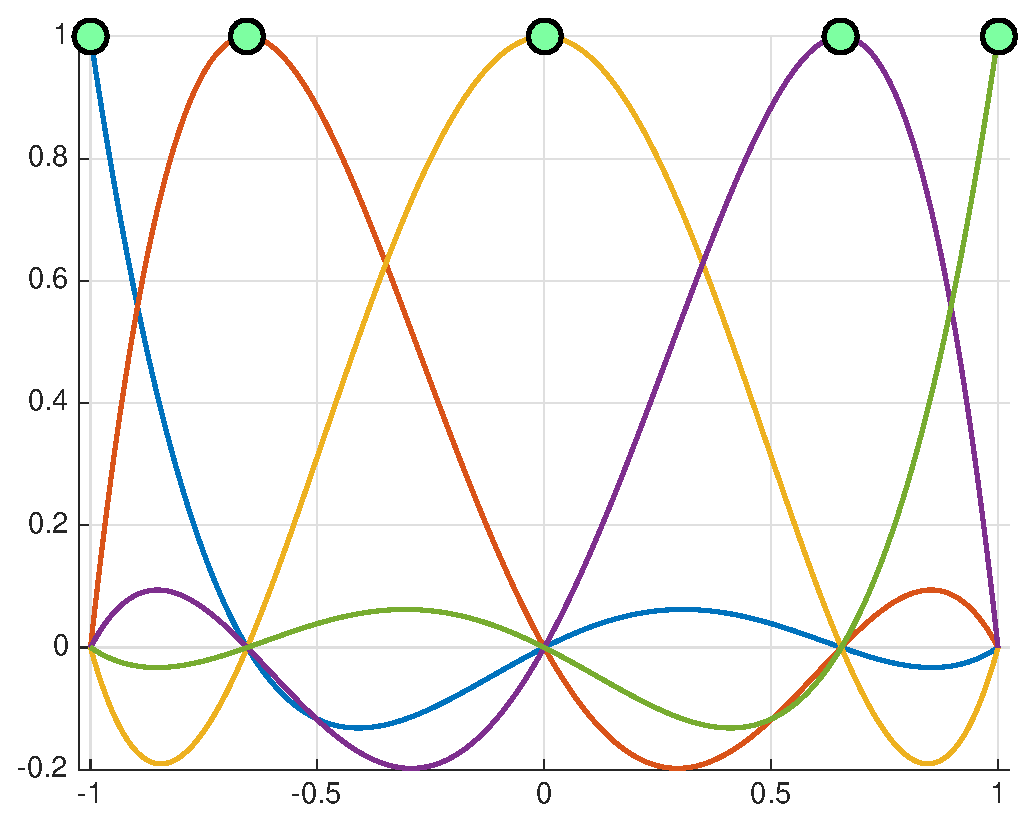
\includegraphics[width=.24\textwidth]{figs/nodal1D.eps}}
\subfloat{\includegraphics[width=.4\textwidth]{figs/nodal2D.png}}
\hspace{.1em}
\subfloat{\includegraphics[width=.31\textwidth]{figs/nodal3D.png}}
\caption*{Lagrange (nodal) bases on a line, triangle, tetrahedron.   }
\end{figure}
%\vspace{.5em}
\begin{itemize}
\item Nodal bases defined implicitly through an orthogonal basis.  
\vspace{.5em}
\item Point locations optimized for interpolation and numerical stability. 
\vspace{.5em}
\item Assume \textbf{affine} tetrahedra, coefficients \textbf{constant} on each element.
%\item Derivative matrices w.r.t.\ reference coordinates $\bm{\widehat{x}} = (r,s,t)$ 
%\[
%\LRp{\mathbf{\widehat{D}}_r}_{ij} = \pd{\ell_j(\bm{\widehat{x}}_i)}{r}{}, \qquad \LRp{\mathbf{\widehat{D}}_s}_{ij} = \pd{\ell_j(\bm{\widehat{x}}_i)}{s}{}, \qquad \LRp{\mathbf{\widehat{D}}_t}_{ij} = \pd{\ell_j(\bm{\widehat{x}}_i)}{t}{}.
%\]
\end{itemize}
}

\frame{
\frametitle{Time-domain nodal DG methods}
%\vspace{-2em}
\begin{columns}
\begin{column}{.55\textwidth}
Given initial condition $u(\mathbf{x},0)$:
\vspace{.25em}
\begin{itemize}
\item<1-> Compute numerical flux at face nodes (\textcolor{red}{non-local}).
\vspace{.25em}
\item<2-> Compute RHS of (\textcolor{blue}{local}) ODE.
\vspace{.25em}
\item<3-> Evolve (\textcolor{blue}{local}) solution using explicit time integration (RK, AB, etc). 
\end{itemize}
\end{column}
\begin{column}{.45\textwidth}
\begin{figure}
\centering
\includegraphics[width=.825\textwidth]{figs/nodal.pdf}
\end{figure}
\end{column}
\end{columns}

%\vspace{1em}
\begin{overlayarea}{\textwidth}{.4\textheight}
\only<1>{\[
\td{\mathbf{u}}{t} = \mathbf{D}_x \mathbf{u} + \sum_{\text{ faces}}\mathbf{L}_f \LRp{\rm \textcolor{red}{flux}}, \qquad \mathbf{L}_f = \mathbf{{M}}^{-1}\mathbf{{M}}_f.
\]
}
\only<2>{
\[
\td{\mathbf{u}}{t} = \underbrace{\mathbf{D}_x \mathbf{u}}_{\text{\textcolor{blue}{Volume kernel}}} + \underbrace{\sum_{\text{ faces}}\mathbf{L}_f \LRp{\rm \textcolor{red}{flux}}}_{\text{\textcolor{blue}{Surface kernel}}}, \qquad \mathbf{L}_f = \mathbf{{M}}^{-1}\mathbf{{M}}_f.
\]
}
\only<3->{
\[
\underbrace{\td{\mathbf{u}}{t}}_{\text{\textcolor{blue}{Update kernel}}} = \underbrace{\mathbf{D}_x \mathbf{u}}_{\text{\textcolor{blue}{Volume kernel}}} + \underbrace{\sum_{\text{ faces}}\mathbf{L}_f \LRp{\rm \textcolor{red}{flux}}}_{\text{\textcolor{blue}{Surface kernel}}}, \qquad \mathbf{L}_f = \mathbf{{M}}^{-1}\mathbf{{M}}_f.
\]
}
\uncover<4->{
\begin{center}
Parallelizable down to individual degrees of freedom!  %\only<5>{For moderate orders\ldots} 
\end{center}
}
\end{overlayarea}
}


%\frame{
%\frametitle{Simplicial elements: affine mappings}
%\begin{itemize}
%\item<1->{Integrals, derivatives w.r.t.\ reference coordinates $\bm{\widehat{x}} = (r,s,t)$% and geometric factors $\pd{rst}{xyz}{}$, $J$.
%\begin{align*}
%\int_{D_k} f(\bm{x})  &= \int_{\widehat{D}} f(\bm{x}\LRp{\bm{\widehat{x}}}) J,\\
%\pd{u}{x}{} &= \pd{u}{r}{}\pd{r}{x}{} + \pd{u}{s}{}\pd{s}{x}{} + \pd{u}{t}{}\pd{t}{x}{}.
%\end{align*}
%}
%\vspace{.1em}
%%\item<3->Mass matrices $=$ scalings of reference mass matrix.
%%\[
%%\mathbf{M}_{ij} = \int_{D_k} \phi_i \phi_j = \int_{\widehat{D}} \phi_i \phi_j J = J \widehat{\mathbf{M}}_{ij}.
%%\]
%%\item<2-> Store reference derivative, lift matrices $\mathbf{\widehat{L}}_f = \mathbf{\widehat{M}}^{-1}\mathbf{\widehat{M}}_f$ for all elements.
%\item<1->For triangles, tetrahedra: exists affine map between $D_k$ and reference element $\widehat{D}$ s.t.\ geometric factors and Jacobian $J$ are \textcolor{red}{constant}.  
%\vspace{1em}
%\item<1-> Requires only geometric factors $+$ reference derivative, lift matrices.
%\[
%\mathbf{D}_x = \pd{r}{x}{} \mathbf{\widehat{D}}_r + \pd{s}{x}{} \mathbf{\widehat{D}}_s + \pd{t}{x}{} \mathbf{\widehat{D}}_t, \qquad  \mathbf{L}_f = \mathbf{{M}}^{-1}\mathbf{{M}}_f = \frac{J^f}{J} \mathbf{\widehat{M}}^{-1}\mathbf{\widehat{M}}_f 
%\]
%\end{itemize}
%\let\thefootnote\relax\footnotetext{\tiny Hesthaven, Warburton, 2008, Nodal discontinuous Galerkin methods: algorithms, analysis, and applications.}
%}
%


%\frame{
%%\frametitle{Polynomial spaces and bases for simplicial elements}
%\frametitle{Building blocks of high order finite elements}
%\begin{itemize}
%\item Approximation space: degree $N$ polynomials
%\[
%\mbb{P}^N = \LRc{r^i s^j t^k, \quad i + j + k \leq N}, \quad \mbb{Q}^N = \LRc{r^i s^j t^k, \quad i, j, k \leq N}.
%\]
%\item $L^2$ polynomial trace inequalities: for $u \in \mbb{P}^N$, face $\widehat{f}\in \partial\widehat{K}$
%\[
%\nor{u}_{L^2(\widehat{f})} \leq C(N) \nor{u}_{L^2(\widehat{K})}
%\]
%Constant $C(N)$ used in stability (SIPDG) and CFL estimates.  
%%\item Planar simplices are affinely related --- constant geometric change of variables factor $J$.  Mass matrix $M$ over any $K$ 
%%\begin{align*}
%%M_{ij} &= \int_{\widehat{K}} \phi_j(x)\phi_i(x) J_K = J_K \widehat{M}.
%%\end{align*}
%\end{itemize}
%\vspace{-.5em}
%\begin{columns}[c]
%\begin{column}{.8\textwidth}
%\begin{itemize}
%\item Lagrange polynomials constructed as a transformation of an orthogonal polynomial basis. 
%\item Nodes optimized for interpolation quality, conditioning.  
%\item Nodal basis reduces cost to compute numerical fluxes.
%\end{itemize}
%\end{column}
%
%\begin{column}{.2\textwidth}
%\vspace{-.5em}
%\begin{figure}
%\centering
%%\only<1>{
%\includegraphics[width=.95\textwidth]{figs/tet_nodes.eps}
%%}
%%\only<2>{
%%\includegraphics[width=.8\textwidth]{figs/nodal_flux.pdf}
%%}
%\end{figure}
%\end{column}
%\end{columns}
%
%\let\thefootnote\relax\footnotetext{\tiny Warburton, Hesthaven 2003. {On the constants in hp-finite element trace inverse inequalities}.}
%\let\thefootnote\relax\footnotetext{\tiny Warburton 2006, {An explicit construction of interpolation nodes on the simplex.}}
%%\let\thefootnote\relax\footnotetext{\tiny Klockner, Warburton, Bridge, Hesthaven 2009, {Nodal discontinuous Galerkin methods on graphics processors}}
%}

%\frame{
%\frametitle{Computational cost of time-domain DG}
%\setcounter{subfigure}{0}
%
%\begin{figure}
%\centering 
%\includegraphics[height=.425\textheight]{figs/scaling.pdf}
%\hspace{.5em}
%\includegraphics[height=.425\textheight]{figs/supercomputer.png}
%\caption*{\scriptsize Parallel scaling of DG with explicit time-stepping (Lucas Wilcox).}
%\end{figure}
%
%\begin{itemize}
%\item<1-> Fixed communication pattern $+$ local work $=$ highly scalable. 
%\vspace{.25em}
%\item<2-> \textcolor{red}{Many dense matrix multiplies per timestep over millions of timesteps!}
%\vspace{.25em}
%\item<2-> Even on hundreds of CPUs: hours for 2D simulations, \textbf{days} for 3D.  
%\end{itemize}
%}


\frame{
\setcounter{subfigure}{0}
\frametitle{Computing with Graphics Processing Units (GPUs)}

\begin{itemize}
\item Scalable but \textit{expensive}: hours for 2D, \textbf{days} for 3D with $\approx 100$ CPUs.
\vspace{.5em}
\item Explicit methods: can replace a small cluster with single GPU.  
\vspace{.5em}
\item Highly energy efficient compared to traditional supercomputers. 
\begin{quote}
\ldots to achieve a [next generation] supercomputer by simply [scaling up] \ldots you'd need a good-size \textcolor{red}{nuclear power plant} next door.  (Kogge 2011)
\end{quote}
\item GPUs reflect broader many-core trends in computing.
%\vspace{.5em}
\begin{figure}
\subfloat[\scriptsize Xeon Phi]{\includegraphics[height=.2\textheight]{figs/phi.png}}
\hspace{2em}
\subfloat[\scriptsize Intel i7 CPU]{\includegraphics[height=.2\textheight]{figs/manycore_cpu.png}}
\end{figure}
\end{itemize}
}

\frame{
\frametitle{DG maps well to many-core (GPU) architectures}
\vspace{-1em}
\begin{figure}
\begin{overlayarea}{\textwidth}{.65\textheight}
\only<1-2>{
\centering
\includegraphics[width=.675\textwidth]{figs/gpu.pdf}
\caption{NVIDIA Maxwell GM204 GPU: 16 cores, 4 SIMD clusters of 32 units.}
}
\only<3->{
\centering
\includegraphics[height=.25\textheight]{figs/airplane_DG.pdf}
\includegraphics[height=.25\textheight]{figs/helicopter.png}
\includegraphics[height=.25\textheight]{figs/airplane.png}\\
\includegraphics[height=.25\textheight]{figs/trifoil.png}
\includegraphics[height=.25\textheight]{figs/car.png}
\includegraphics[height=.25\textheight]{figs/wingflow.png}
\caption{GPU-accelerated simulations of scattering and compressible flow.}
}
\end{overlayarea}
\end{figure}
\vspace{-2.5em}
\only<1-3>{
\begin{itemize}
\item<1-> Thousands of processing elements organized in synchronized groups.  
\item<2-> Stricter memory constraints (data transfer, limited storage), but \ldots 
\item<3-> For DG, reduces computational time from \textbf{days} to \textbf{hours}.%speedups of $\approx 100\times$ observed over serial implementations.
\end{itemize}
}
\let\thefootnote\relax\footnotetext{\tiny Klockner, Warburton, Bridge, Hesthaven 2009, Nodal discontinuous Galerkin methods on graphics processors.}
}

\section{High order Bernstein-Bezier DG methods}

\begin{frame}[noframenumbering]

\frametitle{Outline: improving efficiency of time-domain DG}
    
%Explicit methods: smaller gains compared to other solvers.  This talk: 
%\vspace{.5em}
\begin{itemize}
\item Optimize existing DG methods on GPUs.  
\vspace{.5em}
\item Address simplifying assumptions (constant coefficients, affine tets).
\end{itemize}
\vspace{1em}

\only<1>{
\tableofcontents
}
\only<2>{
\tableofcontents[currentsection]
}

\end{frame}

\frame{
%\frametitle{Nodal tetrahedra at high order}
\frametitle{Computational costs at high orders of approximation}

%\begin{itemize}
%%\item Hexahedra: tensor product structure $\rightarrow$ $O(N^4)$ vs $O(N^6)$ local cost.
%%\item How do (naively implemented) nodal tetrahedra behave at high order?
%\item 
%\end{itemize}
%\vspace{-.25em}
\begin{center}
Problem: (tetrahedral) DG at high orders becomes \textbf{very} expensive!
\end{center}
\vspace{-.5em}
\begin{columns}
\begin{column}{.55\textwidth}
\begin{figure}
\centering
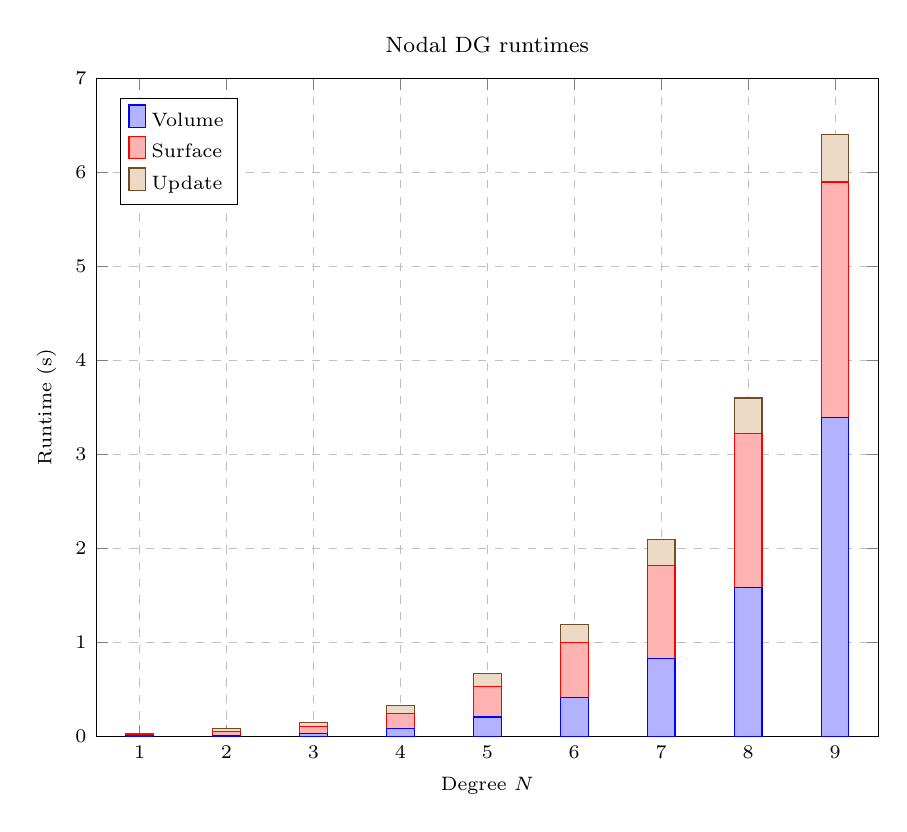
\begin{tikzpicture}
\begin{axis}[
	width=.95\textwidth,
	legend cell align=left,
	%title={Runtime (NPT nodal)},
	title={Nodal DG runtimes},
	xlabel={Degree $N$},
	ylabel={Runtime (s)},
	xmin=.5, xmax=9.5,
	ymin=0,ymax=7,
	ybar stacked,
%	nodes near coords,
	%xmin=.5, xmax=9.5,
	xtick={1,2,3,4,5,6,7,8,9},
	legend pos=north west,
	xmajorgrids=true,
	ymajorgrids=true,
	grid style=dashed,
] 
%nodal runtimes
\addplot coordinates{(1,0.00529)(2,0.0135)(3,0.0302)(4,0.0854)(5,0.206)(6,0.41)(7,0.829)(8,1.58)(9,3.39)};
\addplot coordinates{(1,0.0121)(2,0.0403)(3,0.0722)(4,0.158)(5,0.322)(6,0.587)(7,0.987)(8,1.64)(9,2.51)};
\addplot coordinates{(1,0.009394)(2,0.025607)(3,0.046205)(4,0.080841)(5,0.142045)(6,0.19389)(7,0.27628)(8,0.381)(9,0.5088)};
%\addplot coordinates{(1,0.026784)(2,0.079407)(3,0.148605)(4,0.324241)(5,0.670045)(6,1.19089)(7,2.09228)(8,3.601)(9,6.4088)};

\legend{Volume, Surface, Update}

\end{axis}
\end{tikzpicture}
%\caption*{Per-kernel runtimes for tetrahedra with nodal basis.  Runtimes are recorded for ten RK4 timesteps on a mesh of 98304 elements.}
%\caption*{DG runtimes for 50 timesteps and 98304 elements.}
\caption*{\scriptsize DG runtimes for 50 timesteps, 98304 elements.}
\end{figure}
\end{column}
\begin{column}{.45\textwidth}
\vspace{-2em}
\begin{itemize}
\item Large \textbf{dense} matrices: $O(N^6)$ work per tet.
\vspace{1em}
\item Very high orders usually use tensor-product elements.  
%\vspace{1em}
%\item Tensor-product spectral element methods often use order $N>10$.
\vspace{1em}
\item $O(N^{4})$ vs $O(N^{6})$ cost, but less geometric flexibility.
%\item $O(N^{4})$ vs $O(N^6)$ cost, but less geometric flexibility.
\end{itemize}
\end{column}
\end{columns}
%\let\thefootnote\relax\footnotetext{\tiny Fischer, Ronquist (1994). Spectral element methods for large scale parallel Navier-Stokes calculations.}
%\let\thefootnote\relax\footnotetext{\tiny Sundar et al.\ (2012). Parallel geometric-algebraic multigrid on unstructured forests of octrees.}
}

\frame{
\frametitle{Spectral element methods}
\begin{itemize}
\item Tensor product elements, Gauss-Legendre-Lobatto nodal basis.
\vspace{.25em}
\item $O(N^{d+1})$ vs $O(N^{2d})$ work per element (computing derivatives).
\vspace{.25em}
\item Hexahedral mesh generation more difficult.  
\end{itemize}
\vspace{-.5em}
\begin{figure}
\centering
\subfloat{\includegraphics[width=.4\textwidth]{figs/SEM_stencil_1.pdf}}
\hspace{2em}
\subfloat{\includegraphics[width=.4\textwidth]{figs/SEM_stencil_2.pdf}}
\caption{Spectral element stencils for $N = 7$ (orders $N > 10$ not uncommon!).}
\end{figure}

\let\thefootnote\relax\footnotetext{\tiny Fischer, Ronquist 1994. Spectral element methods for large scale parallel Navier-Stokes calculations.}
\let\thefootnote\relax\footnotetext{\tiny Shepherd and Johnson 2008.  Hexahedral mesh generation constraints.}
}

%\frame{
%\frametitle{Traditional approaches: hybrid meshes}
%\setcounter{subfigure}{0}
%%\vspace{1em}
%\only<1>{
%\vspace{-1em}
%\begin{itemize}
%%\item Tensor-product hexahedra more efficient than tetrahedra. %: $O(N^{4})$ cost (tensor-product), $O(N^{6})$ for tets.
%\item Drawback: hexahedral meshes are less geometrically flexible. 
%\item Solution: use transitional pyramid and wedge elements.
%\end{itemize}
%%\end{center}
%\vspace{-1em}
%\begin{figure}
%\centering 
%\subfloat{\includegraphics[width=.5\textwidth]{figs/hybridpyrmesh1.png}}
%\hspace{1em}
%\subfloat{\includegraphics[width=.35\textwidth]{figs/hybridpyrmesh2.png}}
%%\caption*{Pyramid coupling of hexahedral and tetrahedral meshes}
%\end{figure}
%\vspace{-1em}
%\let\thefootnote\relax\footnotetext{\tiny https://www.sharcnet.ca/Software/TGrid/html/tg/node41.htm}
%\let\thefootnote\relax\footnotetext{\tiny Bergot, Durufle 2013. {Higher-Order Discontinuous Galerkin Method for Pyramidal Elements using Orthogonal Bases}.}
%}
%}
%
%\frame{
%\frametitle{Challenges for hybrid meshes}
%\vspace{-.75em}
%\begin{figure}
%\centering
%\includegraphics[width=.85\textwidth]{figs/hybridmesh_elems.pdf}
%\end{figure}
%\vspace{-1em}
%\begin{itemize}
%\item Recent work: \emph{hex-dominant} unstructured mesh generation.  
%\vspace{.5em}
%\item Challenges: complexity, efficiency depends on mesh composition.
%\end{itemize}
%\let\thefootnote\relax\footnotetext{\tiny Baudouin et al 2014. A frontal approach to hex-dominant mesh generation.}
%\let\thefootnote\relax\footnotetext{\tiny Chan, et al.\ 2015.  {Orthogonal bases for vertex-mapped pyramids}.}
%\let\thefootnote\relax\footnotetext{\tiny Chan, et al.\ 2015.  {GPU-accelerated high order DG methods on hybrid meshes}.}
%}
%

\frame{
\frametitle{High order nodal DG on tetrahedral meshes} %using tetrahedral nodal bases}

\[
\td{\mathbf{u}}{t} = \mathbf{D}_x \mathbf{u} + \sum_{\text{ faces}}\mathbf{L}_f \LRp{\rm flux}, \quad \mathbf{L}_f = \mathbf{{M}}^{-1}\mathbf{{M}}_f.
\]
\vspace{-1em}
\begin{columns}
\begin{column}{.58\textwidth}
\begin{itemize}
\item Nodal bases: reduce the cost of computing numerical fluxes.
\item No special structure in nodal derivative/lift matrices.
\item $O(N^3)$ unknowns in 3D; $O(N^6)$\\ costs for applying \textbf{dense} matrices.  
\end{itemize}
\end{column}
\begin{column}{.42\textwidth}
\begin{figure}
\centering
\includegraphics[width=.875\textwidth]{figs/nodal.pdf}
\end{figure}
\end{column}
\end{columns}
\vspace{1em}
\begin{center}
Derivative and lift matrices depend on the basis:\\
can we choose one that is efficient (and numerically stable)?  
\end{center}
}




\frame{
\frametitle{Bernstein-Bezier bases for finite element methods}

\begin{itemize}
\item Geometry, graphics, Computer Aided Design (CAD).  
\vspace{.5em}
\begin{figure}
\centering
\includegraphics[width=.6\textwidth]{figs/nurbs_bb.png}
\end{figure}
\vspace{.5em}
\item Recent developments: optimal complexity algorithms for quadrature-based integration, assembly of finite element matrices. %
\vspace{.5em}
\item Is Bernstein-Bezier useful for quadrature-free DG methods?
\end{itemize}
\let\thefootnote\relax\footnotetext{\tiny Split multi-span NURBS surfaces into Bezier patches, https://knowledge.autodesk.com} 
\let\thefootnote\relax\footnotetext{\tiny Ainsworth et al.\ 2011. Bernstein-Bezier finite elements of arbitrary order and optimal assembly procedures.}
\let\thefootnote\relax\footnotetext{\tiny Kirby 2011.  Fast simplicial finite element algorithms using Bernstein polynomials.}
}

\frame{
\frametitle{Bernstein-Bezier polynomial bases on simplices}
\vspace{-.5em}
\begin{figure}
\centering
\subfloat{\includegraphics[width=.24\textwidth]{figs/bern1D.pdf}}
\subfloat{\includegraphics[width=.4\textwidth]{figs/bern2D.png}}
\hspace{.1em}
\subfloat{\includegraphics[width=.31\textwidth]{figs/bern3D.png}}
\caption*{Each function attains its maximum at an equispaced lattice point of a $d$-simplex.}
\end{figure}

\begin{itemize}
%\vspace{-.25em}
\item Simple expression in 1D
\[
B^N_i(x) = x^i (1-x)^{N-i}, \qquad 0 \leq x \leq 1.% = \lambda_0^i \lambda_1^j, \qquad i + j = N.
\]
\item Barycentric monomials on a $d$-simplex.  For a tetrahedron,
\[
B^N_{ijkl}(\lambda_0,\lambda_1,\lambda_2,\lambda_3), = \frac{N!}{i!j!k!l!}\lambda_0^i\lambda_1^j\lambda_2^k\lambda_3^l, \quad i+j+k+l = N.
\]
\item Similar structure to nodal basis (vertex, edge, face, interior functions).% similar to the nodal basis.
%\item Efficient differentiation and degree elevation/reduction.
\end{itemize}
}


\frame{
\frametitle{Bernstein-Bezier derivatives and degree elevation in 1D}
\begin{itemize}
\item Simple differentiation of Bernstein polynomials
\[
\pd{B^N_i(x)}{x}{} = N\LRp{B^{N-1}_{i-1}(x) - B^{N-1}_i(x)}.
\]
\item Simple degree elevation of Bernstein polynomials
\[
B^{N-1}_i(x) = \LRp{\frac{N-i}{N}}B^{N}_{i}(x) - \LRp{\frac{i+1}{N}} B^{N}_{i+1}(x).
\]
\item Combine to get expansion of Bernstein derivatives
\[
%\pd{B^N_i(x)}{x}{} = \LRp{N-i+1} B^N_{i-1}(x) +  \LRp{2i-N}B^N_i(x) -  \LRp{i+1} B^N_{i+1}(x).
\pd{B^N_i(x)}{x}{} = a^N_i B^N_{i-1}(x) +  b^N_i B^N_i(x) - c^N_i B^N_{i+1}(x).
\]
Implies 1D derivative matrix $\mathbf{D}_x$ is \textcolor{red}{sparse} (tridiagonal).  
\end{itemize}
}

\frame{
\frametitle{Bernstein-Bezier derivative and degree elevation in 3D}
\setcounter{subfigure}{0}
\begin{itemize}
\item Bernstein-Bezier barycentric differentiation matrices very sparse.% (max 4 nnz/row).
\vspace{.5em}
\item Degree elevation matrices $\mathbf{E}^N_{N-i}$ are sparse (for consecutive degrees).  
\vspace{.5em}
\item Higher degree elevation $\rightarrow$ product of matrices $\mathbf{E}^N_{N-2} = \mathbf{E}^N_{N-1} \mathbf{E}^{N-1}_{N-2}$.
%\item Bernstein-Bezier lift matrix displays some sparsity - can be improved.  
\end{itemize}
\vspace{-.5em}
\begin{figure}
\centering
\subfloat[\scriptsize Derivative matrix w.r.t.\ first barycentric coordinate.]{\includegraphics[height=.475\textheight]{figs/spyD_BB.eps}}
\hspace{2em}
%\subfloat[Bernstein-Bezier lift matrix]{\includegraphics[height=.345\textwidth]{figs/spyLIFT_BB.eps}}
\subfloat[\scriptsize Deg.\ elevation matrix $\mathbf{E}^N_{N-1}$]{\includegraphics[height=.475\textheight]{figs/spyE1.eps}}
\hspace{2em}
\subfloat[\scriptsize$\mathbf{E}^N_{N-2}$]{\includegraphics[height=.475\textheight]{figs/spyE2.eps}}
%\subfloat[$\mathbf{E}^N_{N-3}$]{\includegraphics[height=.45\textheight]{figs/spyE3.eps}}
\end{figure}
}

\frame{
\frametitle{Stencils for Bernstein-Bezier derivative matrices}

\begin{itemize}
\item Stencil sizes at most $(d+1)$ in $d$ dimensions.
\item Compute derivatives w.r.t.\ barycentric coordinates.  
\item Stencil values are identical for each barycentric coordinate.
\end{itemize}
\begin{figure}
\centering
\subfloat[Stencil for $\bm{D}_{\lambda_0}$]{\includegraphics[width=.33\textwidth]{figs/bern_stencil_1.pdf}}
\subfloat[Stencil for $\bm{D}_{\lambda_1}$]{\includegraphics[width=.33\textwidth]{figs/bern_stencil_2.pdf}}
\subfloat[Stencil for $\bm{D}_{\lambda_2}$]{\includegraphics[width=.33\textwidth]{figs/bern_stencil_3.pdf}}
\caption{Bernstein-Bezier stencils for a single node (in \textcolor{red}{red}) $N=7$.}
\end{figure}
}


\frame{
\frametitle{Factorization of the Bernstein lift operator}
\setcounter{subfigure}{0}
\vspace{1em}
The Bernstein-Bezier lift matrix $\mathbf{L}$ admits a factorization of the form
\[
\mathbf{L} = \mathbf{E}_L \LRp{\begin{array}{cccc}\mathbf{L}_0  & & &\\& \mathbf{L}_0 & &\\ & & \mathbf{L}_0 & \\ & & & \mathbf{L}_0\end{array}}. 
\]
\begin{overlayarea}{\textwidth}{.45\textheight}
\vspace{-.5em}
\only<1>{
\begin{figure}
\centering
\subfloat[Lift matrix $\mathbf{L}$]{\includegraphics[height=.23\textwidth]{figs/spyLIFT_BB.eps}}
\hspace{1em}
\subfloat[Lift reduction $\mathbf{E}_L$]{\includegraphics[height=.23\textwidth]{figs/spyEEL_BB.eps}}
\hspace{1em}
\subfloat[$\mathbf{L}_0$]{\includegraphics[height=.23\textwidth]{figs/spyL0_BB.eps}}
\end{figure}
}
\only<2->{
\vspace{-.5em}
\begin{columns}
\begin{column}{.45\textwidth}
\begin{figure}
\centering
\includegraphics[height=.5\textwidth]{figs/spyEEL_BB.eps}
\caption*{\scriptsize $\mathbf{E}_L = \LRs{\begin{array}{c|c|c}
\mathbf{E}_L^1 & \ldots &\mathbf{E}_L^4
\end{array}}$ (4 faces).}
\end{figure}
\end{column}
\begin{column}{.55\textwidth}
\[
\mathbf{E}_L^1 = \LRs{\begin{array}{c}
\mathbf{I} \\
\ell_1\LRp{\mathbf{E}^N_{N-1}}^T \\
%\ell_2\LRp{\mathbf{E}^N_{N-2}}^T \\
\vdots\\
\ell_N\LRp{\mathbf{E}^N_{0}}^T
\end{array}.
}
\]
2D \textcolor{red}{degree reduction} matrices $\LRp{\mathbf{E}^N_{i}}^T$.
\end{column}
\end{columns}
}
\end{overlayarea}
\let\thefootnote\relax\footnotetext{\tiny Chan, Warburton 2015. {GPU-accelerated Bernstein-Bezier DG methods for wave problems}.}
}

\frame{
\frametitle{Bernstein-Bezier lift matrix: optimal complexity application}

\begin{itemize}
\item $\bm{L}$ ``lifts'' numerical fluxes from faces to volume.  
\item Apply $\bm{L}_0$ to face flux, extend to each ``layer'' of the simplex.  
\end{itemize}
\vspace{-1em}
\begin{figure}
\centering
\subfloat[Apply $\bm{L}_0$ to flux to compute face output]{\includegraphics[width=.32\textwidth]{figs/bern_lift_1.pdf}}
\hspace{.1em}
\subfloat[Degree reduce face nodes to compute first layer]{\includegraphics[width=.32\textwidth]{figs/bern_lift_2.pdf}}
\hspace{.1em}
\subfloat[Degree reduce first layer to compute second layer]{\includegraphics[width=.32\textwidth]{figs/bern_lift_3.pdf}}
\caption{An $O(N^{d})$ storage/complexity approach to applying the lift matrix.}  
\end{figure}

\begin{center}
For $N < 6$, currently more efficient to treat $\bm{E}_L$ as a sparse matrix --- irregular data accesses with optimal $O(N^d)$ approach.  
\end{center}
}

%\frame{
%\frametitle{Bernstein-Bezier derivative and lift matrices in 3D}
%\setcounter{subfigure}{0}
%\begin{itemize}
%\item Bernstein-Bezier barycentric differentiation matrices very sparse.% (max 4 nnz/row).
%%\vspace{.5em}
%%\item Degree elevation matrices $\mathbf{E}^N_{N-i}$ are sparse (for consecutive degrees).  
%\vspace{.5em}
%%\item Higher degree elevation $\rightarrow$ product of matrices $\mathbf{E}^N_{N-2} = \mathbf{E}^N_{N-1} \mathbf{E}^{N-1}_{N-2}$.
%\item Bernstein-Bezier lift matrix displays some sparsity - can be improved.  
%\end{itemize}
%\vspace{-.5em}
%\begin{figure}
%\centering
%\subfloat[\scriptsize Derivative matrix w.r.t.\ first barycentric coordinate.]{\includegraphics[height=.475\textheight]{figs/spyD_BB.eps}}
%\hspace{2em}
%\subfloat[Bernstein-Bezier lift matrix]{\includegraphics[height=.345\textwidth]{figs/spyLIFT_BB.eps}}
%%\subfloat[\scriptsize Deg.\ elevation matrix $\mathbf{E}^N_{N-1}$]{\includegraphics[height=.475\textheight]{figs/spyE1.eps}}
%%\hspace{2em}
%%\subfloat[\scriptsize$\mathbf{E}^N_{N-2}$]{\includegraphics[height=.475\textheight]{figs/spyE2.eps}}
%%\subfloat[$\mathbf{E}^N_{N-3}$]{\includegraphics[height=.45\textheight]{figs/spyE3.eps}}
%\end{figure}
%}
%
%\frame{
%\frametitle{Factorization of the Bernstein lift operator}
%\setcounter{subfigure}{0}
%
%\begin{theorem}[Chan, Warburton 2015] 
%The Bernstein-Bezier lift matrix $\mathbf{L}$ admits a factorization of the form
%\[
%\mathbf{L} = \mathbf{E}_L \LRp{\begin{array}{cccc}\mathbf{L}_0  & & &\\& \mathbf{L}_0 & &\\ & & \mathbf{L}_0 & \\ & & & \mathbf{L}_0\end{array}}.%\mathbf{I}\otimes \mathbf{L}_0.
%\]
%\end{theorem} 
%%\only<2->{
%%\begin{columns}
%%\begin{column}{.45\textwidth}
%%\vspace{-1.5em}
%%\begin{figure}
%%\centering
%%\includegraphics[height=.5\textwidth]{figs/spyEEL_BB.eps}
%%\caption*{\scriptsize $\mathbf{E}_L = \LRs{\begin{array}{c|c|c}
%%\mathbf{E}_L^1 & \ldots &\mathbf{E}_L^4
%%\end{array}}$ (4 faces).}
%%\end{figure}
%%\end{column}
%%\begin{column}{.55\textwidth}
%%\[
%%\mathbf{E}_L^1 = \LRs{\begin{array}{c}
%%\mathbf{I} \\
%%\ell_1\LRp{\mathbf{E}^N_{N-1}}^T \\
%%%\ell_2\LRp{\mathbf{E}^N_{N-2}}^T \\
%%\vdots\\
%%\ell_N\LRp{\mathbf{E}^N_{0}}^T
%%\end{array}.
%%}
%%\]
%%2D degree reduction matrices $\LRp{\mathbf{E}^N_{i}}^T$.
%%\end{column}
%%\end{columns}
%%}
%\only<1>{
%\vspace{-1em}
%\begin{figure}
%\centering
%\subfloat[Lift matrix $\mathbf{L}$]{\includegraphics[height=.23\textwidth]{figs/spyLIFT_BB.eps}}
%\hspace{1em}
%\subfloat[Lift reduction $\mathbf{E}_L$]{\includegraphics[height=.23\textwidth]{figs/spyEEL_BB.eps}}
%\hspace{1em}
%\subfloat[$\mathbf{L}_0$]{\includegraphics[height=.23\textwidth]{figs/spyL0_BB.eps}}
%\end{figure}
%}
%\let\thefootnote\relax\footnotetext{\tiny Chan, Warburton 2015. {GPU-accelerated Bernstein-Bezier DG methods for wave problems}.}
%}


\begin{frame}[noframenumbering]
\frametitle{Numerical stability of Bernstein-Bezier DG}
\begin{itemize}
%\item Bernstein polynomials are monomials; numerically stable?
\item Conditioning of derivative, lift matrices comparable to nodal basis.
\[
\kappa(\mathbf{A}) = \frac{\sigma_1}{\sigma_r}
\] 
\item<2-> Comparable long-time growth of (single precision) numerical error.
\end{itemize}
\vspace{-1em}
\begin{figure}
\centering
\begin{overlayarea}{\textwidth}{.6\textheight}
\only<1>{
\subfloat{
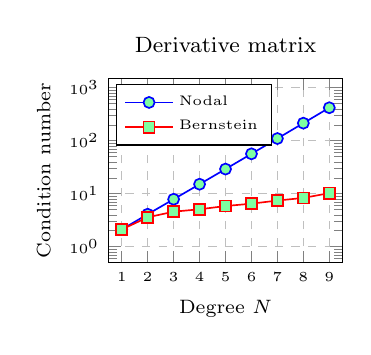
\begin{tikzpicture}
\begin{semilogyaxis}[
    	legend style={font=\tiny},
		ticklabel style = {font=\tiny},
	legend cell align=left,
	width=.375\textwidth,
	title={Derivative matrix},
    xlabel={Degree $N$},
    ylabel={Condition number},
    xmin=.5, xmax=9.5,
    ymin=.5, ymax=1500,
%    ytick={1,10,100,1000},
%    yticklabel={$10^0$,$10^1$,$10^2$,$10^3$},
    xtick={1,2,3,4,5,6,7,8,9},
    legend pos=north west,
    xmajorgrids=true,
    ymajorgrids=true,
    grid style=dashed,
] 
\addplot+[color=blue,mark=*,mark options={fill=markercolor},semithick]
coordinates{(1,2.1166)(2,4.10326)(3,7.8693)(4,15.1262)(5,29.2)(6,56.5943)(7,110.058)(8,214.618)(9,419.473)};
\addplot+[color=red,mark=square*,mark options={fill=markercolor},semithick]
coordinates{(1,2.1166)(2,3.59166)(3,4.58592)(4,5.08895)(5,5.85851)(6,6.49343)(7,7.43361)(8,8.3401)(9,10.2532)};
%\addplot+[color=blue,mark=*,semithick,mark options={fill=markercolor}]
%coordinates{(1,1)(2,3.21827)(3,8.30628)(4,14.1564)(5,22.533)(6,36.2175)(7,58.978)(8,100.128)(9,178.895)};
%\addplot+[color=red,mark=square*,semithick,mark options={fill=markercolor}]
%coordinates{(1,1)(2,1.29099)(3,1.5)(4,1.67332)(5,1.82574)(6,1.96396)(7,2.09165)(8,2.21108)(9,2.32379)};

\legend{Nodal, Bernstein}
\end{semilogyaxis}
\end{tikzpicture}
}
\subfloat{
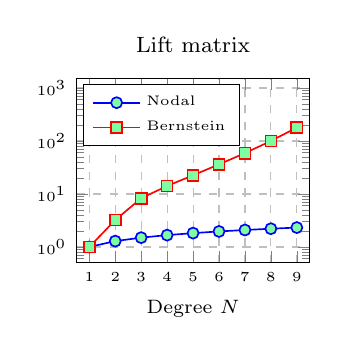
\begin{tikzpicture}
\begin{semilogyaxis}[
	legend cell align=left,
	width=.375\textwidth,
		ticklabel style = {font=\tiny},
title={Lift matrix},
    xlabel={Degree $N$},
%    ylabel={Condition number},
    	legend style={font=\tiny},
    xmin=.5, xmax=9.5,
    ymin=.5, ymax=1500,    
    xtick={1,2,3,4,5,6,7,8,9},
    legend pos=north west,
    xmajorgrids=true,
    ymajorgrids=true,
    grid style=dashed,
] 
\addplot+[color=blue,mark=*,semithick,mark options={fill=markercolor}]
coordinates{(1,1)(2,1.29099)(3,1.5)(4,1.67332)(5,1.82574)(6,1.96396)(7,2.09165)(8,2.21108)(9,2.32379)};
\addplot+[color=red,mark=square*,semithick,mark options={fill=markercolor}]
coordinates{(1,1)(2,3.21827)(3,8.30628)(4,14.1564)(5,22.533)(6,36.2175)(7,58.978)(8,100.128)(9,178.895)};

\legend{Nodal, Bernstein}

\end{semilogyaxis}
\end{tikzpicture}
}
\subfloat{
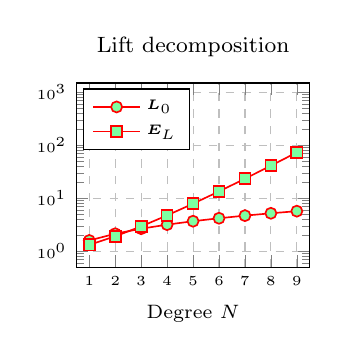
\begin{tikzpicture}
\begin{semilogyaxis}[
	legend cell align=left,
	width=.375\textwidth,
		ticklabel style = {font=\tiny},
       title={Lift decomposition},%$\bm{E}_L$ and $\bm{L}_0$.},
       xlabel={Degree $N$},
%    ylabel={Condition number},
    	legend style={font=\tiny},
    xmin=.5, xmax=9.5,
    ymin=.5, ymax=1500,    
    xtick={1,2,3,4,5,6,7,8,9},
    legend pos=north west,
    xmajorgrids=true,
    ymajorgrids=true,
    grid style=dashed,
] 
\addplot+[color=red,mark=*,semithick,mark options={fill=markercolor}]
coordinates{(1,1.6)(2,2.14286)(3,2.66667)(4,3.18182)(5,3.69231)(6,4.2)(7,4.70588)(8,5.21053)(9,5.71429)};

\addplot+[color=red,mark=square*,semithick,mark options={fill=markercolor}]
coordinates{(1,1.32288)(2,1.91485)(3,2.95099)(4,4.75395)(5,7.90833)(6,13.4748)(7,23.3872)(8,41.1893)(9,73.4078)};

\legend{$\bm{L}_0$, $\bm{E}_L$}

\end{semilogyaxis}
\end{tikzpicture}
}
%\caption*{Condition number $\sigma_1/\sigma_r$ of derivative matrix, lift matrix, and lift decomposition for nodal and Bernstein-Bezier bases.} %for both nodal and Bernstein-Bezier bases.}
\caption*{Condition numbers of matrices for nodal and Bernstein-Bezier bases.} %for both nodal and Bernstein-Bezier bases.}
}
\only<2>{
\subfloat{
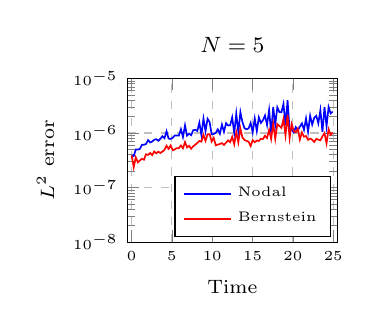
\begin{tikzpicture}
\begin{semilogyaxis}[
	legend cell align=left,
	width=.35\textwidth,
    title={$N = 5$},
    xlabel={Time},
    ylabel={$L^2$ error},
    ticklabel style = {font=\tiny},
    	legend style={font=\tiny},
    xmin=-.5, xmax=25.5,    
    xtick={0,5,10,15,20,25},    
    ymin=1e-8,ymax=1e-5,    
    legend pos=south east,
    xmajorgrids=true,
    ymajorgrids=true,
    grid style=dashed,
] 
\addplot+[color=blue,mark=none,mark options={fill=markercolor},semithick]
coordinates{(0.00942223,3.84995e-07)(0.263822,3.77063e-07)(0.518223,4.99659e-07)(0.772623,4.95252e-07)(1.02702,5.11151e-07)(1.28142,6.06889e-07)(1.53582,6.06564e-07)(1.79022,6.29366e-07)(2.04462,7.41239e-07)(2.29902,6.69313e-07)(2.55342,6.96358e-07)(2.80782,7.51253e-07)(3.06222,7.69608e-07)(3.31662,7.20266e-07)(3.57102,7.8324e-07)(3.82543,8.72844e-07)(4.07983,8.01464e-07)(4.33423,1.07615e-06)(4.58863,7.89313e-07)(4.84303,7.77708e-07)(5.09743,8.17493e-07)(5.35183,8.98188e-07)(5.60623,9.01123e-07)(5.86063,8.94138e-07)(6.11503,1.17259e-06)(6.36943,8.44184e-07)(6.62383,1.38205e-06)(6.87823,8.91514e-07)(7.13263,9.73265e-07)(7.38703,9.11068e-07)(7.64143,1.12352e-06)(7.89583,1.14526e-06)(8.15023,1.08759e-06)(8.40463,1.54808e-06)(8.65903,9.1388e-07)(8.91343,1.83281e-06)(9.16783,1.07909e-06)(9.42223,1.81755e-06)(9.67663,1.5794e-06)(9.93103,9.47185e-07)(10.1854,9.57205e-07)(10.4398,1.00801e-06)(10.6942,1.16644e-06)(10.9486,9.65957e-07)(11.203,1.42273e-06)(11.4574,1.04892e-06)(11.7118,1.51281e-06)(11.9662,1.37004e-06)(12.2206,1.38723e-06)(12.475,1.92986e-06)(12.7294,1.00154e-06)(12.9838,2.26187e-06)(13.2382,1.01886e-06)(13.4926,2.41264e-06)(13.747,1.5811e-06)(14.0014,1.22239e-06)(14.2558,1.16729e-06)(14.5102,1.21446e-06)(14.7646,1.52878e-06)(15.019,1.02512e-06)(15.2734,1.8455e-06)(15.5278,1.0822e-06)(15.7822,1.93168e-06)(16.0366,1.52889e-06)(16.291,1.71152e-06)(16.5454,2.09594e-06)(16.7998,1.39752e-06)(17.0542,2.63722e-06)(17.3086,9.91853e-07)(17.563,2.98945e-06)(17.8174,1.40358e-06)(18.0718,2.95084e-06)(18.3262,2.42357e-06)(18.5806,2.39904e-06)(18.835,3.40491e-06)(19.0894,1.39077e-06)(19.3438,3.97567e-06)(19.5982,1.12321e-06)(19.8526,1.14893e-06)(20.107,1.01862e-06)(20.3614,1.27616e-06)(20.6158,1.12612e-06)(20.8702,1.30673e-06)(21.1246,1.4958e-06)(21.379,1.14004e-06)(21.6334,1.84564e-06)(21.8878,1.04765e-06)(22.1422,2.07671e-06)(22.3966,1.42354e-06)(22.651,1.89572e-06)(22.9054,2.06203e-06)(23.1598,1.50363e-06)(23.4142,2.62205e-06)(23.6686,1.05211e-06)(23.923,2.98076e-06)(24.1774,1.32386e-06)(24.4318,2.97754e-06)(24.6862,2.28985e-06)(24.9406,2.46113e-06)};
\addplot+[color=red,mark=none,semithick,mark options={fill=markercolor}]
coordinates{(0.00942223,3.86948e-07)(0.263822,2.35677e-07)(0.518223,3.58057e-07)(0.772623,2.88983e-07)(1.02702,3.13855e-07)(1.28142,3.36094e-07)(1.53582,3.23459e-07)(1.79022,4.07506e-07)(2.04462,3.95739e-07)(2.29902,4.28878e-07)(2.55342,3.92824e-07)(2.80782,4.58387e-07)(3.06222,4.23612e-07)(3.31662,4.54228e-07)(3.57102,4.30268e-07)(3.82543,4.55962e-07)(4.07983,4.91946e-07)(4.33423,5.83775e-07)(4.58863,5.12281e-07)(4.84303,5.91047e-07)(5.09743,4.83349e-07)(5.35183,5.00045e-07)(5.60623,5.26429e-07)(5.86063,5.28736e-07)(6.11503,5.89948e-07)(6.36943,5.22985e-07)(6.62383,6.82256e-07)(6.87823,5.42033e-07)(7.13263,5.82006e-07)(7.38703,5.13774e-07)(7.64143,5.70022e-07)(7.89583,6.08859e-07)(8.15023,6.58064e-07)(8.40463,7.14815e-07)(8.65903,6.94315e-07)(8.91343,9.30685e-07)(9.16783,7.20271e-07)(9.42223,9.46182e-07)(9.67663,9.52157e-07)(9.93103,6.97769e-07)(10.1854,8.1226e-07)(10.4398,5.92856e-07)(10.6942,6.14142e-07)(10.9486,6.27902e-07)(11.203,6.51575e-07)(11.4574,6.05284e-07)(11.7118,6.63185e-07)(11.9662,7.3344e-07)(12.2206,6.77831e-07)(12.475,8.52744e-07)(12.7294,6.23157e-07)(12.9838,1.03062e-06)(13.2382,6.73812e-07)(13.4926,1.20917e-06)(13.747,8.25663e-07)(14.0014,7.43881e-07)(14.2558,7.17358e-07)(14.5102,6.89299e-07)(14.7646,5.77591e-07)(15.019,7.36187e-07)(15.2734,6.76203e-07)(15.5278,7.28733e-07)(15.7822,7.14491e-07)(16.0366,7.85869e-07)(16.291,7.74484e-07)(16.5454,8.90705e-07)(16.7998,8.08551e-07)(17.0542,1.13944e-06)(17.3086,7.77788e-07)(17.563,1.46731e-06)(17.8174,7.79281e-07)(18.0718,1.45417e-06)(18.3262,1.34498e-06)(18.5806,1.23774e-06)(18.835,1.79806e-06)(19.0894,9.05925e-07)(19.3438,2.14399e-06)(19.5982,8.06568e-07)(19.8526,1.45493e-06)(20.107,1.09129e-06)(20.3614,1.02786e-06)(20.6158,1.19968e-06)(20.8702,7.55967e-07)(21.1246,1.02041e-06)(21.379,8.5471e-07)(21.6334,8.7873e-07)(21.8878,7.47256e-07)(22.1422,7.91899e-07)(22.3966,7.49749e-07)(22.651,6.8323e-07)(22.9054,7.77994e-07)(23.1598,7.53276e-07)(23.4142,7.34561e-07)(23.6686,8.6858e-07)(23.923,9.91957e-07)(24.1774,6.46082e-07)(24.4318,1.16941e-06)(24.6862,9.2726e-07)(24.9406,1.01434e-06)};
\legend{Nodal,Bernstein}
\end{semilogyaxis}
\end{tikzpicture}
}
\subfloat{
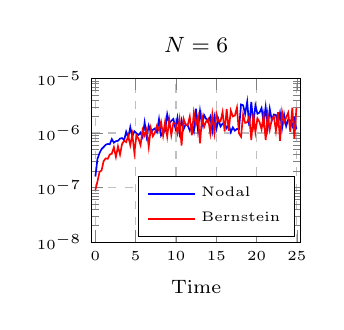
\begin{tikzpicture}
\begin{semilogyaxis}[
	legend cell align=left,
	width=.35\textwidth,
    title={$N = 6$},
    xlabel={Time},
%    ylabel={$L^2$ error},
	legend style={font=\tiny},
	ticklabel style = {font=\tiny},
    xmin=-.5, xmax=25.5,    
    xtick={0,5,10,15,20,25},    
    ymin=1e-8,ymax=1e-5,    
    legend pos=south east,
    xmajorgrids=true,
    ymajorgrids=true,
    grid style=dashed,
] 
\addplot+[color=blue,mark=none,mark options={fill=markercolor},semithick]
coordinates{(0.00942223,1.59337e-07)(0.263822,3.34267e-07)(0.518223,4.27429e-07)(0.772623,5.08211e-07)(1.02702,5.51752e-07)(1.28142,6.07672e-07)(1.53582,6.29049e-07)(1.79022,6.21552e-07)(2.04462,7.72263e-07)(2.29902,6.64154e-07)(2.55342,7.0817e-07)(2.80782,7.17139e-07)(3.06222,7.89352e-07)(3.31662,8.07981e-07)(3.57102,7.35146e-07)(3.82543,1.05491e-06)(4.07983,8.16982e-07)(4.33423,1.2802e-06)(4.58863,8.67775e-07)(4.84303,1.07838e-06)(5.09743,9.90645e-07)(5.35183,9.15434e-07)(5.60623,1.01784e-06)(5.86063,8.36909e-07)(6.11503,1.56378e-06)(6.36943,8.54732e-07)(6.62383,1.3593e-06)(6.87823,1.02163e-06)(7.13263,1.14159e-06)(7.38703,1.21354e-06)(7.64143,1.03392e-06)(7.89583,1.78755e-06)(8.15023,8.94593e-07)(8.40463,1.02153e-06)(8.65903,1.09639e-06)(8.91343,2.20666e-06)(9.16783,1.48997e-06)(9.42223,1.66478e-06)(9.67663,1.80356e-06)(9.93103,1.22332e-06)(10.1854,1.91407e-06)(10.4398,1.00296e-06)(10.6942,1.70362e-06)(10.9486,1.1744e-06)(11.203,1.44629e-06)(11.4574,1.38178e-06)(11.7118,1.10857e-06)(11.9662,1.38231e-06)(12.2206,1.0656e-06)(12.475,2.78469e-06)(12.7294,1.13698e-06)(12.9838,2.5442e-06)(13.2382,1.38374e-06)(13.4926,2.12876e-06)(13.747,1.81043e-06)(14.0014,1.55534e-06)(14.2558,1.97457e-06)(14.5102,1.08551e-06)(14.7646,1.97869e-06)(15.019,1.19172e-06)(15.2734,1.77256e-06)(15.5278,1.3148e-06)(15.7822,1.48718e-06)(16.0366,1.47768e-06)(16.291,1.2237e-06)(16.5454,1.43783e-06)(16.7998,1.03551e-06)(17.0542,1.26394e-06)(17.3086,1.10258e-06)(17.563,1.18557e-06)(17.8174,1.1628e-06)(18.0718,3.33249e-06)(18.3262,3.21885e-06)(18.5806,2.23517e-06)(18.835,3.73378e-06)(19.0894,1.33479e-06)(19.3438,3.7067e-06)(19.5982,1.47732e-06)(19.8526,3.20031e-06)(20.107,2.24583e-06)(20.3614,2.36502e-06)(20.6158,2.86065e-06)(20.8702,1.55678e-06)(21.1246,2.99753e-06)(21.379,1.25036e-06)(21.6334,2.76567e-06)(21.8878,1.70618e-06)(22.1422,2.18238e-06)(22.3966,2.13133e-06)(22.651,1.43188e-06)(22.9054,2.31409e-06)(23.1598,1.22396e-06)(23.4142,2.16151e-06)(23.6686,1.33573e-06)(23.923,1.77086e-06)(24.1774,1.69386e-06)(24.4318,1.32461e-06)(24.6862,1.77528e-06)(24.9406,1.15981e-06)};

\addplot+[color=red,mark=none,semithick,mark options={fill=markercolor}]
coordinates{(0.00942223,9.03235e-08)(0.263822,1.29098e-07)(0.518223,1.93936e-07)(0.772623,2.05495e-07)(1.02702,3.04613e-07)(1.28142,3.41969e-07)(1.53582,3.35877e-07)(1.79022,4.03e-07)(2.04462,4.17363e-07)(2.29902,5.48092e-07)(2.55342,3.64127e-07)(2.80782,5.69421e-07)(3.06222,4.01557e-07)(3.31662,6.27907e-07)(3.57102,7.23612e-07)(3.82543,6.79905e-07)(4.07983,8.85585e-07)(4.33423,5.95572e-07)(4.58863,9.40574e-07)(4.84303,4.33361e-07)(5.09743,8.99871e-07)(5.35183,7.87036e-07)(5.60623,5.99743e-07)(5.86063,1.13867e-06)(6.11503,8.95586e-07)(6.36943,1.18287e-06)(6.62383,5.58382e-07)(6.87823,1.23017e-06)(7.13263,8.70751e-07)(7.38703,1.01032e-06)(7.64143,1.36081e-06)(7.89583,1.10868e-06)(8.15023,1.59034e-06)(8.40463,8.97872e-07)(8.65903,1.63069e-06)(8.91343,8.62928e-07)(9.16783,1.74174e-06)(9.42223,9.13978e-07)(9.67663,1.52592e-06)(9.93103,1.48565e-06)(10.1854,9.99629e-07)(10.4398,1.76496e-06)(10.6942,5.89415e-07)(10.9486,1.81967e-06)(11.203,1.41596e-06)(11.4574,1.38656e-06)(11.7118,1.99872e-06)(11.9662,9.02827e-07)(12.2206,2.36792e-06)(12.475,1.42626e-06)(12.7294,2.01427e-06)(12.9838,6.47492e-07)(13.2382,2.00536e-06)(13.4926,1.29271e-06)(13.747,1.63774e-06)(14.0014,1.80774e-06)(14.2558,9.90484e-07)(14.5102,2.18381e-06)(14.7646,1.00599e-06)(15.019,2.26608e-06)(15.2734,1.61847e-06)(15.5278,1.63951e-06)(15.7822,2.43132e-06)(16.0366,1.06e-06)(16.291,2.76522e-06)(16.5454,1.09777e-06)(16.7998,2.57676e-06)(17.0542,2.01227e-06)(17.3086,2.09511e-06)(17.563,2.92937e-06)(17.8174,9.83384e-07)(18.0718,8.53703e-07)(18.3262,2.17702e-06)(18.5806,1.53061e-06)(18.835,1.56752e-06)(19.0894,2.00298e-06)(19.3438,7.45166e-07)(19.5982,2.20622e-06)(19.8526,1.03844e-06)(20.107,1.8408e-06)(20.3614,1.5947e-06)(20.6158,1.16799e-06)(20.8702,2.11029e-06)(21.1246,7.39822e-07)(21.379,2.16257e-06)(21.6334,1.1482e-06)(21.8878,1.77911e-06)(22.1422,1.99713e-06)(22.3966,1.0908e-06)(22.651,2.40515e-06)(22.9054,7.18939e-07)(23.1598,2.42785e-06)(23.4142,1.5483e-06)(23.6686,1.93166e-06)(23.923,2.35615e-06)(24.1774,1.05027e-06)(24.4318,2.90018e-06)(24.6862,7.87569e-07)(24.9406,2.8777e-06)};

\legend{Nodal,Bernstein}
\end{semilogyaxis}
\end{tikzpicture}
}
\subfloat{
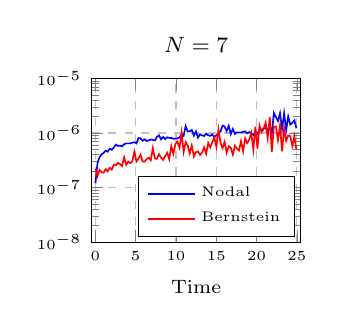
\begin{tikzpicture}
\begin{semilogyaxis}[
	legend cell align=left,
	width=.35\textwidth,
    title={$N = 7$},
    xlabel={Time},
%    ylabel={$L^2$ error},
	legend style={font=\tiny},
	ticklabel style = {font=\tiny},
    xmin=-.5, xmax=25.5,    
    xtick={0,5,10,15,20,25},
    ymin=1e-8,ymax=1e-5,
    legend pos=south east,
    xmajorgrids=true,
    ymajorgrids=true,
    grid style=dashed,
] 
\addplot+[color=blue,mark=none,mark options={fill=markercolor},semithick]
coordinates{(0.00942223,1.18969e-07)(0.263822,2.77767e-07)(0.518223,3.59959e-07)(0.772623,4.05725e-07)(1.02702,4.31285e-07)(1.28142,4.75894e-07)(1.53582,4.5325e-07)(1.79022,5.16143e-07)(2.04462,4.92953e-07)(2.29902,5.42498e-07)(2.55342,6.12257e-07)(2.80782,5.77949e-07)(3.06222,5.87402e-07)(3.31662,5.69701e-07)(3.57103,6.21047e-07)(3.82543,6.44097e-07)(4.07983,6.45598e-07)(4.33423,6.42979e-07)(4.58863,6.67263e-07)(4.84303,6.75895e-07)(5.09743,6.42488e-07)(5.35183,8.06589e-07)(5.60623,8.02611e-07)(5.86063,7.19631e-07)(6.11503,7.66199e-07)(6.36943,7.14729e-07)(6.62383,7.30389e-07)(6.87823,7.60222e-07)(7.13263,7.4791e-07)(7.38703,7.28401e-07)(7.64143,8.46617e-07)(7.89583,9.03316e-07)(8.15023,7.64806e-07)(8.40463,8.49642e-07)(8.65903,7.71403e-07)(8.91343,8.32256e-07)(9.16783,8.11927e-07)(9.42223,8.10728e-07)(9.67663,7.85968e-07)(9.93103,7.86787e-07)(10.1854,7.97513e-07)(10.4398,8.28264e-07)(10.6942,9.47881e-07)(10.9486,8.82563e-07)(11.203,1.33296e-06)(11.4574,1.06488e-06)(11.7118,1.07536e-06)(11.9662,1.13701e-06)(12.2206,8.91041e-07)(12.475,1.07126e-06)(12.7294,8.23971e-07)(12.9838,9.47341e-07)(13.2382,9.00958e-07)(13.4926,8.81191e-07)(13.747,9.73315e-07)(14.0014,9.0684e-07)(14.2558,8.86557e-07)(14.5102,9.4084e-07)(14.7646,8.3838e-07)(15.019,9.12886e-07)(15.2734,9.94088e-07)(15.5278,1.05844e-06)(15.7822,1.3637e-06)(16.0366,1.31046e-06)(16.291,1.08454e-06)(16.5454,1.3592e-06)(16.7998,9.54759e-07)(17.0542,1.18105e-06)(17.3086,9.60576e-07)(17.563,1.02685e-06)(17.8174,1.01463e-06)(18.0718,1.02155e-06)(18.3262,1.04755e-06)(18.5806,1.07173e-06)(18.835,9.83862e-07)(19.0894,1.03728e-06)(19.3438,9.79466e-07)(19.5982,9.21262e-07)(19.8526,1.05401e-06)(20.107,9.61514e-07)(20.3614,1.15439e-06)(20.6158,1.13152e-06)(20.8702,1.22349e-06)(21.1246,1.23295e-06)(21.379,1.11801e-06)(21.6334,1.40854e-06)(21.8878,9.43115e-07)(22.1422,2.32792e-06)(22.3966,1.96131e-06)(22.651,1.66291e-06)(22.9054,2.30348e-06)(23.1598,1.18047e-06)(23.4142,2.30781e-06)(23.6686,1.1242e-06)(23.923,2.00211e-06)(24.1774,1.43003e-06)(24.4318,1.5372e-06)(24.6862,1.70213e-06)(24.9406,1.21646e-06)};

\addplot+[color=red,mark=none,semithick,mark options={fill=markercolor}]
coordinates{(0.00942223,2.20193e-07)(0.263822,1.61922e-07)(0.518223,2.10928e-07)(0.772623,1.90155e-07)(1.02702,1.86747e-07)(1.28142,2.17112e-07)(1.53582,1.97358e-07)(1.79022,2.29712e-07)(2.04462,2.1406e-07)(2.29902,2.63323e-07)(2.55342,2.59024e-07)(2.80782,2.83009e-07)(3.06222,2.69977e-07)(3.31662,2.48711e-07)(3.57103,3.5815e-07)(3.82543,2.61698e-07)(4.07983,2.98939e-07)(4.33423,2.79248e-07)(4.58863,3.02818e-07)(4.84303,4.56847e-07)(5.09743,2.99679e-07)(5.35183,3.38105e-07)(5.60623,4.00296e-07)(5.86063,2.99816e-07)(6.11503,2.99638e-07)(6.36943,3.32252e-07)(6.62383,3.51669e-07)(6.87823,3.16237e-07)(7.13263,5.2494e-07)(7.38703,3.39399e-07)(7.64143,3.36897e-07)(7.89583,4.07952e-07)(8.15023,3.5457e-07)(8.40463,3.20798e-07)(8.65903,3.73246e-07)(8.91343,4.33288e-07)(9.16783,3.31251e-07)(9.42223,5.74808e-07)(9.67663,4.11773e-07)(9.93103,6.30739e-07)(10.1854,6.95452e-07)(10.4398,5.3708e-07)(10.6942,1.02049e-06)(10.9486,4.49329e-07)(11.203,6.78877e-07)(11.4574,5.89683e-07)(11.7118,4.23455e-07)(11.9662,5.88911e-07)(12.2206,3.7196e-07)(12.475,4.44646e-07)(12.7294,4.5932e-07)(12.9838,3.97968e-07)(13.2382,4.3413e-07)(13.4926,5.4413e-07)(13.747,4.16291e-07)(14.0014,6.56205e-07)(14.2558,5.44616e-07)(14.5102,6.85559e-07)(14.7646,8.21004e-07)(15.019,5.58738e-07)(15.2734,1.16051e-06)(15.5278,6.5633e-07)(15.7822,5.26931e-07)(16.0366,6.84698e-07)(16.291,4.3554e-07)(16.5454,5.72016e-07)(16.7998,5.35723e-07)(17.0542,4.01191e-07)(17.3086,5.83645e-07)(17.563,5.16393e-07)(17.8174,4.76094e-07)(18.0718,7.11568e-07)(18.3262,4.59762e-07)(18.5806,7.97498e-07)(18.835,6.5153e-07)(19.0894,7.53359e-07)(19.3438,1.00457e-06)(19.5982,4.95595e-07)(19.8526,1.30958e-06)(20.107,5.17539e-07)(20.3614,1.37688e-06)(20.6158,1.03074e-06)(20.8702,1.17885e-06)(21.1246,1.54962e-06)(21.379,7.99616e-07)(21.6334,1.96826e-06)(21.8878,4.47481e-07)(22.1422,1.30195e-06)(22.3966,1.31541e-06)(22.651,7.44483e-07)(22.9054,1.37148e-06)(23.1598,4.62151e-07)(23.4142,1.20753e-06)(23.6686,7.15283e-07)(23.923,8.99061e-07)(24.1774,8.75244e-07)(24.4318,5.76796e-07)(24.6862,8.70818e-07)(24.9406,4.92085e-07)};

\legend{Nodal,Bernstein}
\end{semilogyaxis}
\end{tikzpicture}
}
%\caption*{Growth of (single precision) $L^2$ error over time for nodal and Bernstein-Bezier bases. } %Both $N$ and the number of elements are taken to be sufficiently large such that the approximation error is at machine (single) precision.}
\caption*{Evolution of $L^2$ error (acoustics) for nodal and Bernstein-Bezier bases. } %Both $N$ and the number of elements are taken to be sufficiently large such that the approximation error is at machine (single) precision.}
\label{fig:errOverTime}
}
\end{overlayarea}
\end{figure}

\end{frame}


%% ========

\frame{
\frametitle{GPU runtime comparison of BBDG and nodal DG}

\vspace{-.5em}
\begin{center}
Bernstein-Bezier DG achieves $\approx 2\times$ speedup at moderate orders,\\ and up to $\approx 6\times$ speedup at high orders.
\end{center}
%\begin{center}
%Bernstein-Bezier DG achieves $\approx 2\times$ speedup at moderate orders,\\ and up to $4\times$ speedup at high orders.
%\end{center}
\vspace{-1em}
\begin{figure}
\centering
\only<1>{
\hspace{-1em}
\subfloat{
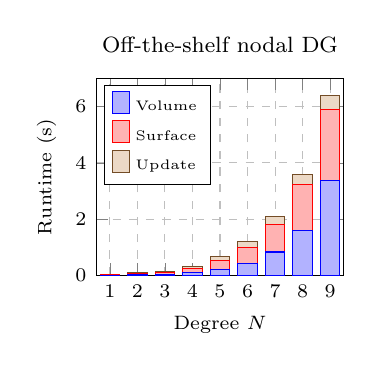
\begin{tikzpicture}
\begin{axis}[
	width=.39\textwidth,
	legend cell align=left,
	title={Off-the-shelf nodal DG},
	xlabel={Degree $N$},
	ylabel={Runtime (s)},
	xmin=.5, xmax=9.5,
	ymin=0,ymax=7,
	ybar stacked,
	    bar width=7pt,
	legend style={font=\tiny},	
	xtick={1,2,3,4,5,6,7,8,9},
	legend pos=north west,
	xmajorgrids=true,
	ymajorgrids=true,
	grid style=dashed,
] 
%nodal runtimes
\addplot coordinates{(1,0.00529)(2,0.0135)(3,0.0302)(4,0.0854)(5,0.206)(6,0.41)(7,0.829)(8,1.58)(9,3.39)};
\addplot coordinates{(1,0.0121)(2,0.0403)(3,0.0722)(4,0.158)(5,0.322)(6,0.587)(7,0.987)(8,1.64)(9,2.51)};
\addplot coordinates{(1,0.009394)(2,0.025607)(3,0.046205)(4,0.080841)(5,0.142045)(6,0.19389)(7,0.27628)(8,0.381)(9,0.5088)};

\legend{Volume, Surface, Update}

\end{axis}
\end{tikzpicture}
}
\subfloat{
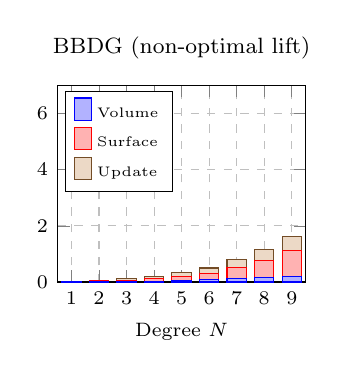
\begin{tikzpicture}
\begin{axis}[
	width=.39\textwidth,
	legend cell align=left,
	title={BBDG (non-optimal lift)},
	xlabel={Degree $N$},
	legend style={font=\tiny},	
%	ylabel={Runtime (s)},
	xmin=.5, xmax=9.5,
	ymin=0,ymax=7,
	ybar stacked,
	    bar width=7pt,
	xtick={1,2,3,4,5,6,7,8,9},
	legend pos=north west,
	xmajorgrids=true,
	ymajorgrids=true,
	grid style=dashed,
] 
%bern runtimes
\addplot 
coordinates{(1,0.00564)(2,0.0119)(3,0.0203)(4,0.034)(5,0.0593)(6,0.0791)(7,0.112)(8,0.155)(9,0.204)};
\addplot 
coordinates{(1,0.0148)(2,0.0276)(3,0.0459)(4,0.0842)(5,0.149)(6,0.227)(7,0.42)(8,0.614)(9,0.912)};
\addplot 
coordinates{(1,0.0093767)(2,0.0255921)(3,0.04623)(4,0.081)(5,0.14229)(6,0.194133)(7,0.277041)(8,0.38163)(9,0.50694)};

\legend{Volume, Surface, Update}

\end{axis}
\end{tikzpicture}
}
\subfloat{
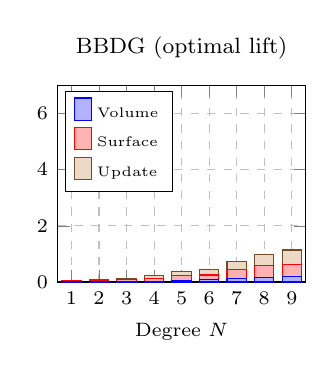
\begin{tikzpicture}
\begin{axis}[
	width=.39\textwidth,
	legend cell align=left,
	title={BBDG (optimal lift)},
	xlabel={Degree $N$},
	legend style={font=\tiny},	
%	ylabel={Runtime (s)},
	xmin=.5, xmax=9.5,
	ymin=0,ymax=7,
	ybar stacked,
	    bar width=7pt,
	xtick={1,2,3,4,5,6,7,8,9},
	legend pos=north west,
	xmajorgrids=true,
	ymajorgrids=true,
	grid style=dashed,
] 
%bern runtimes
\addplot 
coordinates{(1,0.00564)(2,0.0119)(3,0.0203)(4,0.034)(5,0.0593)(6,0.0791)(7,0.112)(8,0.155)(9,0.204)};
\addplot 
coordinates{(1,3.45E-02)(2,5.15E-02)(3,6.61E-02)(4,1.03E-01)(5,1.76E-01)(6,1.73E-01)(7,3.32E-01)(8,4.48E-01)(9,4.31E-01)};
\addplot 
coordinates{(1,0.0093767)(2,0.0255921)(3,0.04623)(4,0.081)(5,0.14229)(6,0.194133)(7,0.277041)(8,0.38163)(9,0.50694)};

\legend{Volume, Surface, Update}

\end{axis}
\end{tikzpicture}
}
%\caption*{Per-kernel runtimes for nodal and Bernstein-Bezier bases.  Runtimes are recorded for ten RK4 timesteps on a mesh of 98304 elements.}
%\caption*{Kernel runtimes for Naive nodal, Blocked nodal, and Bernstein-Bezier DG implementations (50 RHS evaluations, 98304 elements).}
%\caption*{Kernel runtimes for Standard nodal, Blocked nodal, and Bernstein-Bezier DG implementations (50 RHS evaluations, 98304 elements).}
%\caption*{DG runtimes for 50 timesteps, 98304 elements.}
}

% maybe comment out? speedup
\only<2>{
\subfloat{
\begin{tikzpicture}
\begin{axis}[
	width=.425\textwidth,
	legend cell align=left,
	%title={BB speedup over Naive nodal},
	title={BB speedup (non-opt.\ lift) over nodal},
	xlabel={Degree $N$},
	ylabel={Speedup},
	xmin=.5, xmax=9.5,
	ymin=0,ymax=8,%17.5,	
        ybar=2*\pgflinewidth,
    bar width=3pt,
	xtick={1,2,3,4,5,6,7,8,9},
	ymin=0,
	legend pos=north west,
	legend style={font=\tiny},
	ymajorgrids=true,
	grid style=dashed,
] 
%speedup V/S
\addplot table[x=N, y=V] from \runtimeNaive;
\addplot table[x=N, y=S] from \runtimeNaive;
\addplot table[x=N, y=T] from \runtimeNaive;
%\addplot table[x=N, y=Vopt] from \datatable;
\addplot+[draw=black,line legend, very thick,smooth,dashed] coordinates{(0,1)(10,1)};
%\legend{Volume, Surface, Total, Reference (no speedup)}
\legend{Volume, Surface, Total}%, No speedup}
\end{axis}
\end{tikzpicture}
}
\subfloat{
\begin{tikzpicture}
\begin{axis}[
	width=.425\textwidth,
	legend cell align=left,
	%title={BB speedup over Naive nodal},
	title={BB speedup (optimal lift) over nodal},
	xlabel={Degree $N$},
	ylabel={Speedup},
	xmin=.5, xmax=9.5,
	ymin=0,ymax=8,%17.5,	
        ybar=2*\pgflinewidth,
    bar width=3pt,
	xtick={1,2,3,4,5,6,7,8,9},
	ymin=0,
	legend pos=north west,
	legend style={font=\tiny},
	ymajorgrids=true,
	grid style=dashed,
] 
%speedup V/S
\addplot table[x=N, y=V] from \runtimeOptNaive;
\addplot table[x=N, y=S] from \runtimeOptNaive;
\addplot table[x=N, y=T] from \runtimeOptNaive;
%\addplot table[x=N, y=Vopt] from \datatable;
\addplot+[draw=black,line legend, very thick,smooth,dashed] coordinates{(0,1)(10,1)};

%\legend{Volume, Surface, Total, Reference (no speedup)}
\legend{Volume, Surface, Total}%, No speedup}
\end{axis}
\end{tikzpicture}

}

%\caption*{Ratio of runtimes of volume/surface kernels and total RHS evaluation using a Bernstein-Bezier basis instead of nodal polynomials.}
%\caption*{Speedups achieved over nodal DG by using a Bernstein-Bezier basis.}
}
%\caption*{Bernstein-Bezier DG achieves $\approx 2\times$ speedup at moderate orders,\\ and up to $4\times$ speedup at high orders.}
\end{figure}
\only<1>{\vspace{-.25em}}
\only<2>{\vspace{-.5em}}
\[
\underbrace{\td{\mathbf{u}}{t}}_{\text{Update kernel}} = \underbrace{\mathbf{D}_x \mathbf{u}}_{\text{Volume kernel}} + \underbrace{\sum_{\text{ faces}}\mathbf{L}_f \LRp{\rm flux}}_{\text{Surface kernel}}, \quad \mathbf{L}_f = \mathbf{{M}}^{-1}\mathbf{{M}}_f.
\]
}

%\frame{
%\frametitle{Future work: hybrid meshes}
%\begin{itemize}
%\item Pyramid basis: defined on cube, mapped using Duffy transform.
%\begin{align*}
%B^N_{ijk}(a,b,c) = B^{N-k}_i(a)B^{N-k}_j(b)B^N_k(c).
%\end{align*}
%\end{itemize}
%\begin{columns}
%\begin{column}{.6\textwidth}
%\begin{itemize}
%%\item Hex, wedge bases defined as tensor products of lines, triangle.
%%\vspace{1em}
%\item Preserves Bernstein-Bezier properties (positivity, partition of unity).
%\vspace{1em}
%\item Can use Bernstein-Bezier pyramids in 3D exact geometry meshing.
%\end{itemize}
%\end{column}
%\begin{column}{.4\textwidth}
%\begin{figure}
%\centering
%\includegraphics[width=.95\textwidth]{figs/bern_pyr.png}
%\end{figure}
%\end{column}
%\end{columns}
%\vspace{.5em}
%
%\let\thefootnote\relax\footnotetext{\tiny Chan, Warburton 2015.  A short note on a Bernstein-Bezier basis for the pyramid. }
%\let\thefootnote\relax\footnotetext{\tiny Michoski, Chan, Engvall, Evans 2015.  Foundations of the Blended Isogeometric Discontinuous Galerkin (BIDG) Method. }
%}


\section{Weight-adjusted DG: heterogeneous media}

\begin{frame}[noframenumbering]
    \frametitle{Outline}
    \tableofcontents[currentsection]
\end{frame}

\frame{
\frametitle{Energy stable discontinuous Galerkin formulations}

\begin{itemize}
\item Model problem: acoustic wave equation
\begin{align*}
\frac{1}{c^2}\pd{p}{t}{} = \Div \bm{u}, \qquad \pd{\bm{u}}{t}{} = \Grad p
\end{align*}
\item (Local) formulation with penalty fluxes 
\begin{align*}
\int_{D^k}\frac{1}{c^2}\pd{p}{t}{} q &= \int_{D^k} \Div \bm{u} q  + \frac{1}{2}\int_{\partial D^k} \LRp{\jump{\bm{u}}\cdot{\bm{n}} + \tau_p\jump{p}} q\\
\int_{D^k}\pd{\bm{u}}{t}{} \bm{v} &= \int_{D^k} \Grad p \cdot \bm{v} + \frac{1}{2}\int_{\partial D^k} \LRp{\jump{p} + \tau_u\jump{\bm{u}}\cdot\bm{n}} \bm{v}
\end{align*}
\item \textcolor{red}{High order accuracy}, semi-discrete \textcolor{red}{energy stability}
\[
\pd{}{t}{}\LRp{\sum_{k} \int_{D^k} \frac{p^2}{c^2} + \LRb{\bm{u}}^2} = -\sum_k\int_{\partial D^k} \tau_p\jump{p}^2 +  \tau_u\jump{\bm{u}\cdot\bm{n}}^2 \leq 0.
\]
\end{itemize}
}

\frame{
\frametitle{High order approximation of media and geometry}
\setcounter{subfigure}{0}
\begin{itemize}
\item Efficient implementation on \textbf{simplicial} meshes: \only<1>{$c^2$}\only<2->{\textcolor{red}{$c^2$}} piecewise constant, non-curved meshes (\only<1>{$J, J^f$}\only<2->{\textcolor{red}{$J, J^f$}} piecewise constant).  
\vspace{.1em}
\begin{align*}
\only<1>{
\int_{D^k}\frac{1}{c^2}\pd{p}{t}{} q &= \int_{D^k} \Div \bm{u} q  + \frac{1}{2}\int_{\partial D^k} \LRp{\jump{\bm{u}}\cdot{\bm{n}} + \tau_p\jump{p}} q\\
\int_{D^k}\pd{\bm{u}}{t}{} \bm{v} &= \int_{D^k} \Grad p \cdot \bm{v} + \frac{1}{2}\int_{\partial D^k} \LRp{\jump{p} + \tau_u\jump{\bm{u}}\cdot\bm{n}} \bm{v}
}
\only<2>{
\int_{\widehat{D}}\textcolor{red}{\frac{1}{c^2}}\pd{p}{t}{} q \textcolor{red}{J} &= \int_{\widehat{D}} \Div \bm{u} q\textcolor{red}{J}  + \frac{1}{2}\int_{\partial \widehat{D}} \LRp{\jump{\bm{u}}\cdot{\bm{n}} + \tau_p\jump{p}} q\textcolor{red}{J^f}\\
\int_{\widehat{D}}\pd{\bm{u}}{t}{} \bm{v} \textcolor{red}{J} &= \int_{\widehat{D}} \Grad p \cdot \bm{v}\textcolor{red}{J} + \frac{1}{2}\int_{\partial \widehat{D}} \LRp{\jump{p} + \tau_u\jump{\bm{u}}\cdot\bm{n}} \bm{v}\textcolor{red}{J^f}
}
\only<3>{
\textcolor{red}{\frac{J}{c^2}}\int_{\widehat{D}}\pd{p}{t}{} q  &= \textcolor{red}{J}\int_{\widehat{D}} \Div \bm{u} q  + \textcolor{red}{J^f}\frac{1}{2}\int_{\partial \widehat{D}} \LRp{\jump{\bm{u}}\cdot{\bm{n}} + \tau_p\jump{p}} q\\
\textcolor{red}{J}\int_{\widehat{D}}\pd{\bm{u}}{t}{} \bm{v}  &= \textcolor{red}{J}\int_{\widehat{D}} \Grad p \cdot \bm{v} + \textcolor{red}{J^f}\frac{1}{2}\int_{\partial \widehat{D}} \LRp{\jump{p} + \tau_u\jump{\bm{u}}\cdot\bm{n}} \bm{v}
}
\end{align*}
\vspace{.1em}
\item Spurious reflections for low order approximations of media, geometry.
\end{itemize}
\vspace{-.75em}
\begin{figure}
\subfloat[Mesh and exact $c^2$]{\includegraphics[width=.31\textwidth]{figs/c2WADG.png}}
\hspace{.2em}
\subfloat[Piecewise const.\ $c^2$]{\includegraphics[width=.275\textwidth]{figs/p0WADG.png}}
\hspace{.2em}
\subfloat[High order $c^2$]{\includegraphics[width=.275\textwidth]{figs/pNWADG.png}}
\end{figure}
}

%\frame{
%\frametitle{High order models of heterogeneous media}
%\begin{itemize}
%\item Acoustic wave equation in heterogeneous media
%\[
%\frac{1}{c^2(\bm{x})}\pd{p}{t}{2} - \Delta p = 0.
%\]
%\item $c^2(\bm{x})$ often assumed piecewise constant for efficiency.
%\vspace{.5em}
%\item Discontinuities in $c^2(\bm{x})$ can result in spurious reflections.
%\end{itemize}
%
%\begin{figure}
%\subfloat[Mesh and exact $c^2$]{\includegraphics[width=.33\textwidth]{figs/c2WADG.png}}
%\hspace{.2em}
%\subfloat[Piecewise constant $c^2$]{\includegraphics[width=.31\textwidth]{figs/p0WADG.png}}
%\hspace{.2em}
%\subfloat[High order $c^2$]{\includegraphics[width=.31\textwidth]{figs/pNWADG.png}}
%\end{figure}
%}

%\frame{
%\frametitle{Extension to heterogeneous media, curvilinear meshes}
%\begin{itemize}
%\item Acoustic wave equation in heterogeneous media
%\[
%\frac{1}{c^2(\bm{x})}\pd{p}{t}{2} - \Delta p = 0.
%\]
%%\vspace{.5em}
%\item \only<1,3->{Curvilinear}\only<2>{\textcolor{red}{Curvilinear}} meshes and wave propagation in \only<1-2,4>{heterogeneous media}\only<3>{\textcolor{red}{heterogeneous media}}:  DG mass matrices have spatially varying weight
%\begin{overlayarea}{\textwidth}{.26\textheight}
%\vspace{-1.25em}
%\only<1,4>{
%\begin{align*}
%\LRp{\bm{M}_{w}}_{ij} &= \int_{\widehat{D}}\phi_i \phi_j w(x),\\
%\td{}{t}\bm{M}_{w} \bm{u} &= \text{right hand side}.
%\end{align*}
%}
%\only<2>{
%\begin{align*}
%\LRp{\bm{M}_{w}}_{ij} &= \int_{\widehat{D}}\phi_i \phi_j \textcolor{red}{J(x)}, \\
%\td{}{t}\bm{M}_{\textcolor{red}{J}} \bm{u} &= \text{right hand side}.
%\end{align*}
%}
%\only<3>{
%\begin{align*}
%\LRp{\bm{M}_{w}}_{ij} &= \int_{\widehat{D}}\phi_i \phi_j \textcolor{red}{\frac{J}{c^{2}(x)}}, \\
%\td{}{t}\bm{M}_{\textcolor{red}{J/c^2}} \bm{u} &= \text{right hand side}.
%\end{align*}
%}
%\end{overlayarea}
%%\vspace{.0em}
%\item Inherits continuous energy stability with respect to weighted $L^2$ norm, but requires $\bm{M}_w^{-1}$ \only<1-3>{over each element}\only<4>{\textcolor{red}{over each element}}.
%\end{itemize}
%}

\frame{
\frametitle{Weighted mass matrices}
\begin{itemize}
\item Spatially varying weights appear in DG mass matrices
\[
\only<1,4->{\int_{\widehat{D}}{\frac{1}{c^2}}\pd{p}{t}{} q {J} = \text{pressure RHS}, \qquad \int_{\widehat{D}}\pd{\bm{u}}{t}{} \bm{v} {J} = \text{velocity RHS}}
\only<2>{\int_{\widehat{D}}{\frac{1}{c^2}}\pd{p}{t}{} q \textcolor{red}{J} =  \text{pressure RHS}, \qquad \int_{\widehat{D}}\pd{\bm{u}}{t}{} \bm{v} \textcolor{red}{J} = \text{velocity RHS}}
\only<3>{\int_{\widehat{D}}\textcolor{red}{\frac{1}{c^2}}\pd{p}{t}{} q \textcolor{red}{J} =  \text{pressure RHS}, \qquad \int_{\widehat{D}}\pd{\bm{u}}{t}{} \bm{v} \textcolor{red}{J} = \text{velocity RHS}}
\]
\item \only<1,3->{Curvilinear}\only<2>{\textcolor{red}{Curvilinear}} meshes and wave propagation in \only<1-2,4>{heterogeneous media}\only<3>{\textcolor{red}{heterogeneous media}} 
\begin{overlayarea}{\textwidth}{.26\textheight}
\vspace{-1.25em}
\only<1,4>{
\begin{align*}
\LRp{\bm{M}_{w}}_{ij} &= \int_{\widehat{D}}\phi_i \phi_j w(x),\\
\td{}{t}\bm{M}_{w} \bm{u} &= \text{right hand side}.
\end{align*}
}
\only<2>{
\begin{align*}
\LRp{\bm{M}_{w}}_{ij} &= \int_{\widehat{D}}\phi_i \phi_j \textcolor{red}{J(x)}, \\
\td{}{t}\bm{M}_{\textcolor{red}{J}} \bm{u} &= \text{right hand side}.
\end{align*}
}
\only<3>{
\begin{align*}
\LRp{\bm{M}_{w}}_{ij} &= \int_{\widehat{D}}\phi_i \phi_j \textcolor{red}{\frac{J}{c^{2}(x)}}, \\
\td{}{t}\bm{M}_{\textcolor{red}{J/c^2}} \bm{u} &= \text{right hand side}.
\end{align*}
}
\end{overlayarea}
\item Inherits \textbf{high order accuracy} and \textbf{energy stability} with respect to a weighted $L^2$ norm, but requires $\bm{M}_w^{-1}$ explicitly \only<1-3>{over each element}\only<4>{\textcolor{red}{over each element}}.
\vspace{.5em}
\item On-the-fly assembly + inversion or pre-computation and \textcolor{red}{storage}.
\end{itemize}
}

%\frame{
%\frametitle{Memory limitations for accelerator architectures}
%%\vspace{-1em}
%\begin{table}
%\centering                                                                                   
%\begin{tabular}{| c | c | c | c |}
%\hline
%Model & Approx Cost & Year & Memory \\
%\hline
%GeForce GTX280 & \$70? (old) & 2008  & 1 GB \\
%\hline 
%Tesla K20  & \$2800 & 2012  & 5 GB \\
%\hline 
%Tesla K40 & \$3500 & 2014  & 12 GB \\
%\hline 
%Tesla P100 & \$7400 & 2016  & 16 GB \\
%\hline 
%\end{tabular}
%\label{table:arch}
%\end{table}
%Memory costs of DG (\emph{single precision}, 3D tetrahedra, 1M elements):
%\begin{table}
%\centering                                                                                   
%\begin{tabular}{| c | c | c | c | c |}
%\hline
%Order $N$ & $N=1$ & $N=3$ & $N=5$ & $N=7$ \\
%\hline
%Block matrix $M^{-1}$ & .298 GB  & \textcolor{red}{3.2 GB}  & \textcolor{red}{25.08 GB} & \textcolor{red}{115.2 GB} \\
%\hline
%Solution dofs & .075 GB  & .16 GB  & .448 GB & .96 GB \\
%\hline 
%\end{tabular}
%\label{table:cost}
%\end{table}
%\begin{center}
%Large storage, data movement costs at high order if $w = w(\bm{x})$.
%\end{center}
%}

\frame{
\frametitle{Weight-adjusted DG: convergence and implementation}
\begin{itemize}
\item \textcolor{red}{Weight-adjusted DG (WADG)}: energy stable approximation of weighted mass matrix  
\[
\td{}{t}\bm{M}_{w}\bm{u} \approx \td{}{t}\textcolor{red}{{\bm{M}} \LRp{{\bm{M}}_{1/w}}^{-1} {\bm{M}}} \bm{u} = \text{right hand side}.
\]
\item WADG \textit{a-priori} estimates: standard DG $O\LRp{h^{N+1/2}}$ convergence of $L^2$ error based on optimal weighted projection estimate:
\begin{align*}
&\nor{u - P_w u}_{L^2} \leq C h^{N+1}  \nor{w}_{W^{N+1,\infty}} \nor{\frac{\sqrt{J}}{w}}_{L^{\infty}} \nor{u}_{W^{N+1,2}}.
\end{align*}
\item Bypasses inverse of weighted matrix $\LRp{\bm{M}_{w}}^{-1}$ 
\[
\LRp{{\bm{M}} \LRp{{\bm{M}}_{1/w}}^{-1}{\bm{M}}}^{-1} = {\bm{M}}^{-1} {{\bm{M}}}_{1/w} {\bm{M}}^{-1}.
\]
\end{itemize}
}

\frame{
\frametitle{A non-intrusive and low-storage implementation}
\begin{itemize}
\item Operator evaluation reuses implementation for $w=1$
\begin{align*}
{\bm{M}} \LRp{{\bm{M}}_{1/w}}^{-1} {\bm{M}} \td{\bm{U}}{t} &= \bm{A}_h \bm{U} \\
\rightarrow \LRp{{\bm{M}}_{1/w}}^{-1} {\bm{M}} \td{\bm{U}}{t} &= \underbrace{\bm{M}^{-1}\bm{A}_h \bm{U} }_{\text{RHS for }w = 1}
\end{align*}
%\vspace{.25em}
\item Low storage: matrix-free application of $\bm{M}^{-1}{\bm{M}}_{1/w}$.  
\[
\LRp{\bm{M}}^{-1} {\bm{M}}_{1/w}\text{RHS} = \underbrace{\widehat{\bm{M}}^{-1} \bm{V}_q^T W}_{\bm{P}_q} {\rm diag}\LRp{1/w} \bm{V}_q \LRp{\text{RHS}}.
\]
\item Non-intrusive: modify RHS locally before update.  For non-curved meshes, can combine with \textit{optimal complexity} RHS evaluation.\footnotemark
\end{itemize}

\let\thefootnote\relax\footnotetext{\tiny Chan, Warburton 2015.  {GPU-accelerated Bernstein-Bezier discontinuous Galerkin methods for wave propagation}.}
}


\frame{
\frametitle{Weight-adjusted DG: not locally conservative}

\begin{itemize}
\item \textcolor{red}{Con:} loss of local conservation for $w(x) \not\in P^N$!
\vspace{1em}
\item \textcolor{blue}{Pro:} superconvergence of conservation error
\begin{align*}
%&\LRb{\int_{\widehat{D}} w p(\bm{x},t) - \int_{\widehat{D}} T_{1/w}^{-1} p(\bm{x},t)} \\
\text{Conservation error}
&\leq C \textcolor{red}{h^{2N+2}} \nor{w}_{W^{N+1,\infty}}\nor{p}_{W^{N+1,2}}
\end{align*}
where $C$ depends on mesh quality and max/min values of $w$.
\vspace{1em}
\item \textcolor{blue}{Pro:} can restore local conservation with rank-1 update (Shermann-Morrison).
\end{itemize}
}


\frame{
\frametitle{Acoustic wave equation: heterogeneous media}
\setcounter{subfigure}{0}

\begin{figure}
\centering
\only<1>{
\subfloat[$c^2(x,y)$]{
\includegraphics[width=.325\textwidth]{figs/cfun.png}
}
\hspace{1em}
\subfloat[Standard DG]{
\includegraphics[width=.325\textwidth]{figs/cmass_wave.png}
}}
\only<2>{
\subfloat[$c^2(x,y)$]{
\includegraphics[width=.325\textwidth]{figs/cfun.png}
}
\hspace{1em}
\subfloat[Weighted-adjusted DG]{
\includegraphics[width=.325\textwidth]{figs/cproj_wave.png}
}}
\caption{Standard vs.\ weight-adjusted DG with spatially varying $c^2$ containing both smooth variations and a discontinuity.}
\end{figure}
}


\frame{
\frametitle{Acoustics, variable coefficients: $L^2$ errors}
\setcounter{subfigure}{0}
\vspace{.5em}
Smooth wavefield $c^2(x,y) = 1 + \frac{1}{2}\sin(\pi x)\sin(\pi y)$
\only<1>{
\begin{table}
\centering                                                                                   
\begin{tabular}{c||c|c|c|c|}
\hline                                                   
 & $h = 1$ & $h = 1/2$ & $h = 1/4$ & $h = 1/8$\\ 
\hline                                                   
DG $N = 1$ &   2.13e-01 & 6.25e-02 & 1.64e-02 & 4.19e-03 \\
\hline
WADG $N = 1$ &  2.05e-01 & 5.99e-02 & 1.62e-02 & 4.18e-03 \\
%\hhline{=====}                              
\hline \\ \hline
DG $N = 2$ &  3.01e-02 & 3.60e-03 & 4.21e-04 & 5.07e-05 \\
\hline                                                   
WADG $N = 2$ &  2.89e-02 & 3.54e-03 & 4.18e-04 & 5.07e-05 \\
%\hhline{|=||=|=|=|=|}                                   
\hline \\ \hline
DG $N = 3$ &   6.10e-03 & 3.33e-04 & 2.04e-05 & 1.22e-06 \\
\hline                                                   
WADG $N = 3$ &   8.69e-03 & 3.47e-04 & 2.03e-05 & 1.22e-06 \\
%\hhline{|=||=|=|=|=|}                            
\hline \\ \hline
DG $N = 4$ &  6.61e-04 & 2.12e-05 & 6.39e-07 & 1.94e-08 \\
\hline                                                   
WADG $N = 4$ & 1.09e-03 & 2.27e-05 & 6.30e-07 & 1.93e-08 \\
\hline                                                   
\end{tabular}

\caption{Convergence of standard, weight-adjusted DG to a manufactured solution.}
\label{table:manusol}
\end{table}
}
\only<2>{
\begin{table}
\centering
%\subfloat[Standard DG, reference solution (spectral method)]{
\begin{tabular}{c||c|c|c|c|}
\hline                                                   
 & $h = 1$ & $h = 1/2$ & $h = 1/4$ & $h = 1/8$\\ 
\hline                                                   
DG $N = 1$ &   2.48e-01 & 7.58-02 & 1.69e-02 & 4.46e-03 \\
\hline                                                
WADG $N = 1$ &  2.50e-01 & 7.72e-02 & 1.69e-02 & 4.47e-03 \\
%\hhline{|=||=|=|=|=|}
\hline \\ \hline
DG $N = 2$ &  5.95e-02 & 9.95e-03 & 1.10e-03 & 1.22e-04 \\
\hline                                                   
WADG $N = 2$ &  6.09e-02 & 1.02e-02 & 1.10e-03 & 1.22e-04 \\
%\hhline{|=||=|=|=|=|}
\hline \\ \hline
DG $N = 3$ &   2.29e-02 & 1.98e-03 & 9.52e-05 & 6.56e-06 \\
\hline                                                   
WADG $N = 3$ &   1.98e-02 & 1.98e-03 & 9.52e-05 & 6.56e-06 \\
%\hhline{|=||=|=|=|=|}                              
\hline \\ \hline
DG $N = 4$ &  4.90e-03 & 3.01e-04 & 1.78e-05 & 7.27e-07 \\
\hline                                                   
WADG $N = 4$ & 4.64e-03 & 3.02e-04 & 1.78e-05 & 7.28e-07 \\
\hline 
\end{tabular}
%}\\
%\subfloat[Weighted DG, reference solution (spectral method)]{
%\begin{tabular}{|c||c|c|c|c|}
%\hline                                                   
% & $h = 1$ & $h = 1/2$ & $h = 1/4$ & $h = 1/8$\\ 
%\hline 
%\end{tabular}
%}
\caption{Convergence to a reference solution ($N = 100$ spectral method).}
\label{table:rates}
\end{table}
}
}


\frame{
\frametitle{Acoustics, variable coefficients: convergence}
\setcounter{subfigure}{0}

\begin{table}
\centering
\subfloat[Rates of convergence to manufactured solution]{
\begin{tabular}{|c||c|c|c|c|}
\hline                                                   
 & $N = 1$ & $N = 2$ & $N = 3$ & $N = 4$\\ 
\hline                                                   
DG&       1.9220  &     3.0752     &      4.0440      &      5.0446    \\
\hline                                                   
WADG &  1.9211 &     3.0629     &    4.0752    &   5.0990\\
\hline 
\end{tabular}
}\\
\subfloat[Rates of convergence to reference solution]{
\begin{tabular}{|c||c|c|c|c|}
\hline                                                   
 & $N = 1$ & $N = 2$ & $N = 3$ & $N = 4$\\ 
\hline                                                   
DG &   1.8256  &      3.1796  &    3.8589    &  4.6171         \\
\hline                                                   
WADG &  1.8425 &      3.1807  & 3.8583   & 4.6128 \\
\hline 
\end{tabular}
}
%\caption{Estimated convergence rates for manufactured, reference solutions.}
\end{table}

\begin{center}
Observed $L^2$ rates between optimal $O(h^{N+1})$ and estimated $O(h^{N+1/2})$.
\end{center}
}

\subsection{Curvilinear meshes}

\begin{frame}[noframenumbering]
    \frametitle{Outline}
    \tableofcontents[currentsection,currentsubsection]
\end{frame}

\frame{
\frametitle{Weight-adjusted DG for curvilinear meshes}

%\begin{figure}
%\centering
%%\captionsetup[subfigure]{labelformat=empty}
%\subfloat{\includegraphics[width=.23\textwidth]{figs/curved_mesh.png}}
%\hspace{.5em}
%\setcounter{subfigure}{0}
%\subfloat{\includegraphics[width=.3\textwidth]{figs/curved_mesh.png}}
%\end{figure}

\begin{itemize}
\item Weight-adjusted $L^2$ projection $\tilde{P}_N$ on curved domains
\[
\tilde{P}_N(u) \coloneqq P_N\LRp{\frac{1}{J}P_N\LRp{uJ}}.
\]
where $P_N$ is the $L^2$ projection onto the reference element.
\vspace{1em}
\item $L^2$ estimates for weight-adjusted projection:
\begin{align*}
\nor{u - \tilde{P}_N u}_{L^2\LRp{D^k}} &\lesssim \nor{\frac{1}{\sqrt{J}}}_{L^{\infty}}^2 \textcolor{red}{\nor{J}_{W^{N+1,\infty}\LRp{D^k}}} h^{N+1}\nor{u}_{W^{N+1,2}\LRp{D^k}}.
\end{align*}
\vspace{.1em}
\item High order Sobolev norm of $J$ - implies that convergence can suffer for non-smooth mappings.
\end{itemize}
}

\frame{
\frametitle{Behavior of weight-adjusted $L^2$ projection}

\only<1-2>{
Comparison with $L^2$ projection and Low-Storage Curvilinear DG
\[
\tilde{\phi}_i = \frac{\phi_i}{\sqrt{J}}, \qquad \bm{M}_{ij} = \int_{D^k} \tilde{\phi}_j\tilde{\phi}_i J = \int_{\widehat{D}} \phi_j\phi_i = \widehat{\bm{M}}_{ij}.
\]
\vspace{-2em}
}

\begin{figure}
\begin{overlayarea}{\textwidth}{.6\textheight}
\centering
\only<1>{
\subfloat{
\includegraphics[width=.37\textwidth]{figs/arnoldmesh1.png}
}
\subfloat{
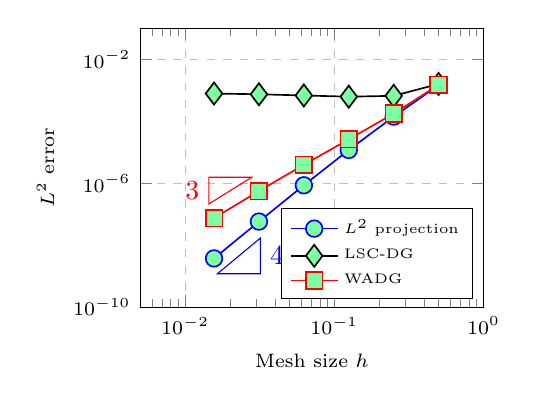
\begin{tikzpicture}
\begin{loglogaxis}[
	legend cell align=left,
	        legend style={font=\tiny},	
	width=.49\textwidth,
    xlabel={Mesh size $h$},
    ylabel={$L^2$ error},
    xmin=.005, xmax=1,
    ymin=1e-10, ymax=1e-1,
    legend pos=south east,
    xmajorgrids=true,
    ymajorgrids=true,
    grid style=dashed,
] 
% adding this 2x because pgfplots dashes the line for some reason...
\addplot[color=blue,mark=*,mark size=3,semithick, mark options={fill=markercolor}]
coordinates{(0.5,0.00145465)(0.25,0.000140693)(0.125,1.17949e-05)(0.0625,8.58138e-07)(0.03125,5.78543e-08)(0.015625,3.75483e-09)};
\addplot[color=black,mark=diamond*,mark size=4,semithick, mark options={fill=markercolor}]
coordinates{(0.5,0.00159198)(0.25,0.000658818)(0.125,0.000619747)(0.0625,0.000677173)(0.03125,0.00073964)(0.015625,0.000782687)};
\addplot[color=red,mark=square*,mark size=3,semithick, mark options={fill=markercolor}]
coordinates{(0.5,0.00148852)(0.25,0.000176325)(0.125,2.60169e-05)(0.0625,3.94602e-06)(0.03125,5.58752e-07)(0.015625,7.47639e-08)};
\logLogSlopeTriangleFlip{0.325}{0.125}{0.37}{3}{red};
\logLogSlopeTriangle{0.35}{0.125}{0.12}{4}{blue};

\legend{$L^2$ projection, LSC-DG, WADG}
\end{loglogaxis}
\end{tikzpicture}
}
\caption{Arnold-type mesh with $\nor{J}_{W^{N+1,\infty}} = O(h^{-1})$ for $N = 3$.}
}
\only<2>{
\subfloat{
\includegraphics[width=.37\textwidth]{figs/randunif1.png}
}
\subfloat{
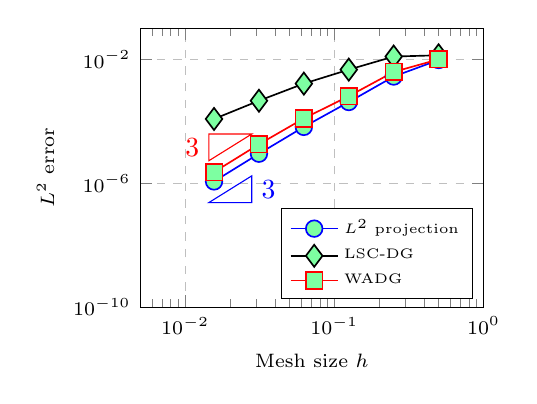
\begin{tikzpicture}
\begin{loglogaxis}[
	legend cell align=left,
	        legend style={font=\tiny},
	width=.49\textwidth,
    xlabel={Mesh size $h$},
    ylabel={$L^2$ error},
    xmin=.005, xmax=1,
    ymin=1e-10, ymax=1e-1,
    legend pos=south east,
    xmajorgrids=true,
    ymajorgrids=true,
    grid style=dashed,
] 
\addplot[color=blue,mark=*,mark size=3,semithick, mark options={fill=markercolor}]
coordinates{(0.5,0.00943375)(0.25,0.00276313)(0.125,0.000415615)(0.0625,6.56974e-05)(0.03125,8.95162e-06)(0.015625,1.14109e-06)};
\addplot[color=black,mark=diamond*,mark size=4,semithick, mark options={fill=markercolor}]
coordinates{(0.5,0.0134065)(0.25,0.012209)(0.125,0.004612)(0.0625,0.00163555)(0.03125,0.000458367)(0.015625,0.00011822)};
\addplot[color=red,mark=square*,mark size=3,semithick, mark options={fill=markercolor}]
coordinates{(0.5,0.00990795)(0.25,0.00389737)(0.125,0.00064227)(0.0625,0.000123078)(0.03125,1.80455e-05)(0.015625,2.28866e-06)};
\logLogSlopeTriangleFlip{0.325}{0.125}{0.525}{3}{red};
\logLogSlopeTriangle{0.325}{0.125}{0.375}{3}{blue};

\legend{$L^2$ projection, LSC-DG, WADG}
\end{loglogaxis}
\end{tikzpicture}
}
\caption{Curvilinear mesh constructed through random perturbation for $N = 3$.}
}
\only<3>{
\vspace{-2em}
High order convergence \textcolor{red}{slowed} by growth of $\nor{J}_{W^{N+1,\infty}} = O(h^N)$.
\vspace{1em}

\subfloat{
\includegraphics[width=.37\textwidth]{figs/curvarnold2ref.png}
}
\subfloat{
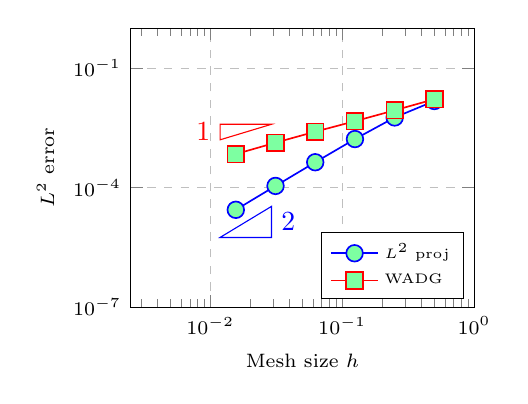
\begin{tikzpicture}
\begin{loglogaxis}[
legend style={font=\tiny},
	legend cell align=left,
	width=.49\textwidth,
    xlabel={Mesh size $h$},
    ylabel={$L^2$ error},
    xmin=.0025, xmax=1,
    ymin=1e-7, ymax=1e-0,
    legend pos=south east,
    xmajorgrids=true,
    ymajorgrids=true,
    grid style=dashed,
] 
% adding this 2x because pgfplots dashes the line for some reason...
\addplot[color=blue,mark=*,mark size=3,semithick, mark options={fill=markercolor}]
coordinates{(0.5,0.0149174)(0.25,0.00576658)(0.125,0.00165616)(0.0625,0.000433839)(0.03125,0.000110389)(0.015625,2.78024e-05)};
%\addplot[color=black,mark=diamond*,mark size=4,semithick, mark options={fill=markercolor}]
%coordinates{(0.5,0.018737)(0.25,0.0147278)(0.125,0.0117761)(0.0625,0.0110991)(0.03125,0.0112431)(0.015625,0.0114663)};
\addplot[color=red,mark=square*,mark size=3,semithick, mark options={fill=markercolor}]
coordinates{(0.5,0.0165783)(0.25,0.00872368)(0.125,0.00464969)(0.0625,0.00253621)(0.03125,0.00134518)(0.015625,0.000695124)};
\logLogSlopeTriangleFlip{0.41}{0.15}{0.6}{1}{red};
\logLogSlopeTriangle{0.41}{0.15}{0.25}{2}{blue};

%\node at (axis cs:.03,2.1e-07) {$a = 10^{-1}$};

%\legend{$L^2$ proj, LSC-DG, WADG}
\legend{$L^2$ proj, WADG}
\end{loglogaxis}
\end{tikzpicture}
}
\caption{Moderately warped curved Arnold-type mesh for $N = 3$.}
}
\only<4>{
\vspace{-2em}
High order convergence is \textcolor{red}{stalled} by growth of $\nor{J}_{W^{N+1,\infty}} = O(h^{N+1})$.
\vspace{1em}

\subfloat{
\includegraphics[width=.37\textwidth]{figs/curvarnold1ref.png}
}
\subfloat{
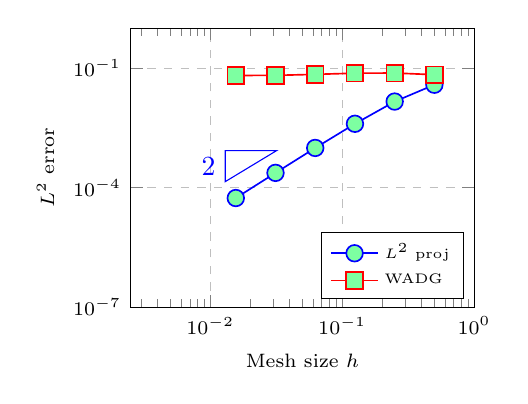
\begin{tikzpicture}
\begin{loglogaxis}[
legend style={font=\tiny},
	legend cell align=left,
	width=.49\textwidth,
    xlabel={Mesh size $h$},
    ylabel={$L^2$ error},
    xmin=.0025, xmax=1,
    ymin=1e-7, ymax=1e-0,
    legend pos=south east,
    xmajorgrids=true,
    ymajorgrids=true,
    grid style=dashed,
] 
\addplot[color=blue,mark=*,mark size=3,semithick, mark options={fill=markercolor}]
coordinates{(0.5,0.038232)(0.25,0.0144542)(0.125,0.00400233)(0.0625,0.000991275)(0.03125,0.000234827)(0.015625,5.4896e-05)};
%\addplot[color=black,mark=diamond*,mark size=4,semithick, mark options={fill=markercolor}]
%coordinates{(0.5,0.0579895)(0.25,0.052133)(0.125,0.0462352)(0.0625,0.0434683)(0.03125,0.0394193)(0.015625,0.032696)};
\addplot[color=red,mark=square*,mark size=3,semithick, mark options={fill=markercolor}]
coordinates{(0.5,0.0681969)(0.25,0.0751338)(0.125,0.0744307)(0.0625,0.0695447)(0.03125,0.0656228)(0.015625,0.0653247)};
%\logLogSlopeTriangleFlip{0.3}{0.125}{0.475}{1}{red};
\logLogSlopeTriangleFlip{0.425}{0.15}{0.45}{2}{blue};

%\node at (axis cs:.03,2.1e-07) {$a = 10^{-1}$};

%\legend{$L^2$ proj, LSC-DG, WADG}
\legend{$L^2$ proj, WADG}
\end{loglogaxis}
\end{tikzpicture}
}
\caption{Heavily warped curved Arnold-type mesh for $N = 3$.}
}

\end{overlayarea}

\end{figure}
}

\frame{
\frametitle{Curvilinear meshes: two-dimensional verification}
%\vspace{-1.5em}
\vspace{1em}
Energy stability: quadrature-based skew-symmetric formulation. 
\begin{figure}
\centering
%\captionsetup[subfigure]{labelformat=empty}
\subfloat{\includegraphics[width=.375\textwidth]{figs/curved_mesh.png}}
\hspace{.5em}
\setcounter{subfigure}{0}
\subfloat[$L^2$ errors for $N = 2,3,4$]{

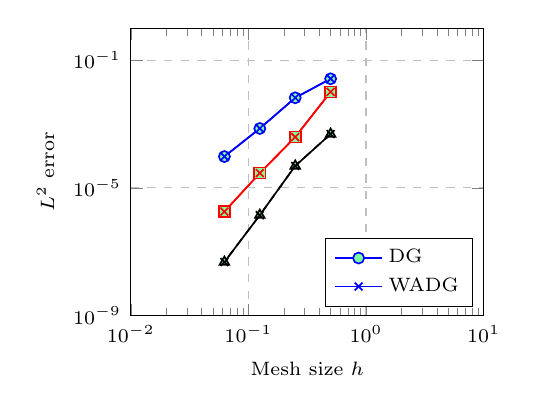
\begin{tikzpicture}
\begin{loglogaxis}[
	legend cell align=left,
	width=.5\textwidth,
%    title={Convergence},
    xlabel={Mesh size $h$},
    ylabel={$L^2$ error},
    xmin=.01, xmax=10,
    ymin=1e-9, ymax=1,        
    legend pos=south east,
    xmajorgrids=true,
    ymajorgrids=true,
    grid style=dashed,
] 
\addplot+[color=blue,mark=*,mark options={fill=markercolor},semithick]
coordinates{(0.5,0.026045)(0.25,0.00661508)(0.125,0.000722446)(0.0625,9.5217e-05)};
\addplot+[color=blue,mark=x,mark options={solid,fill=markercolor},semithick]
coordinates{(0.5,0.0260431)(0.25,0.00661506)(0.125,0.000722445)(0.0625,9.5217e-05)};

\addplot+[color=red,mark=square*,mark options={fill=markercolor},semithick]
coordinates{(0.5,0.0101239)(0.25,0.000387682)(0.125,2.88879e-05)(0.0625,1.78875e-06)};
\addplot+[color=red,mark=x,mark options={solid,fill=markercolor},semithick]
coordinates{(0.5,0.0101238)(0.25,0.000387682)(0.125,2.88879e-05)(0.0625,1.78875e-06)};

\addplot+[color=black,mark=triangle*,mark options={fill=markercolor},semithick]
coordinates{(0.5,0.000483144)(0.25,4.84164e-05)(0.125,1.38952e-06)(0.0625,4.71587e-08)};
\addplot+[color=black,mark=x,mark options={solid,fill=markercolor},semithick]
coordinates{(0.5,0.000483096)(0.25,4.84162e-05)(0.125,1.38952e-06)(0.0625,4.71587e-08)};
\legend{DG,WADG}
\end{loglogaxis}
\end{tikzpicture}
}
\caption{Optimal $L^2$ convergence rates observed for curvilinear meshes.  }
\end{figure}
}

\frame{
\frametitle{Curvilinear meshes: DG eigenvalues (circular domain)}
\vspace{-1.5em}
\begin{figure}
\centering
\subfloat[Central fluxes]{
\includegraphics[width=.36\textwidth]{figs/eigstau0.png}
}
\subfloat[${\rm Im}\LRp{\lambda_i}$ for central fluxes]{
\includegraphics[width=.36\textwidth]{figs/eigstau0imag.png}
}\\
\subfloat[Upwind fluxes]{
\includegraphics[width=.36\textwidth]{figs/eigstau1.png}
}
%\caption{Spectra of discretized wave equation using DG and WADG for $N=3$.  Both central ($\tau = 0$) and dissipative ($\tau = 1$) numerical fluxes are shown.}
\end{figure}
}

%\frame{
%\frametitle{Three-dimensional curvilinear meshes}
%\setcounter{subfigure}{0}
%\begin{figure}
%\centering
%\subfloat[Planar initial mesh]{
%\includegraphics[width=.325\textwidth]{figs/spherePlanar1.png}
%}
%\hspace{.25em}
%\subfloat[Curved initial mesh]{
%\includegraphics[width=.3\textwidth]{figs/sphereCurved1.png}
%}
%\hspace{.25em}
%\subfloat[Curved refined mesh]{
%\includegraphics[width=.3\textwidth]{figs/sphereCurved2.png}
%}
%\caption{Meshes constructed using Gordon-Hall blending.}
%\end{figure}
%}
%

%\frame{
%\frametitle{Convergence on three-dimensional curvilinear meshes}
%
%\begin{figure}
%\centering
%%\vspace{-1em}
%\subfloat{
%\raisebox{2em}{
%\includegraphics[width=.35\textwidth]{figs/sphereCurved2.png}
%}
%}
%\hspace{.5em}
%\subfloat{
%\begin{tikzpicture}
%\begin{loglogaxis}[
%	legend cell align=left,
%	legend style={font=\tiny},
%	width=.575\textwidth,
%%    xlabel={Degrees of freedom},
%    xlabel={Mesh size $h$},
%    ylabel={$L^2$ error},
%%    xmin=400, xmax=2e6,
%    xmin=5e-2, xmax=1.25,
%    ymin=1e-9, ymax=.1,        
%    legend pos=south east,
%    xmajorgrids=true,
%    ymajorgrids=true,
%    grid style=dashed,
%    cycle list name=color list]
%] 
%\addplot+[color=blue,mark=*,mark options={fill=markercolor},semithick]
%coordinates{(1,0.0138761)(0.499567,0.00549824)(0.1682,9.03376e-05)(0.0830612,7.85662e-06)};
%
%\addplot+[color=red,mark=square*,mark options={fill=markercolor},semithick]
%coordinates{(1,0.00407636)(0.499567,0.000325115)(0.1682,3.81903e-06)(0.0830612,2.07829e-07)};
%
%\addplot+[color=black,mark=triangle*,mark options={fill=markercolor},semithick]
%coordinates{(1,0.000836237)(0.499567,4.83058e-05)(0.1682,1.00745e-07)};
%
%\addplot+[color=magenta,mark=diamond*,mark options={fill=markercolor},semithick]
%coordinates{(1,0.000232785)(0.499567,3.13379e-06)(0.1682,7.82233e-09)};
%
%\logLogSlopeTriangleFlip{0.3}{0.15}{0.52}{3}{blue};
%\logLogSlopeTriangleFlip{0.3}{0.15}{0.32}{4}{red};
%\logLogSlopeTriangleFlip{0.475}{0.125}{0.26}{5}{black};
%\logLogSlopeTriangle{0.55}{0.15}{0.1}{5.5}{magenta};
%
%%\logLogSlopeTriangleNeg{0.85}{0.15}{0.55}{-1}{blue};
%%\logLogSlopeTriangleNeg{0.85}{0.15}{0.39}{-4/3}{red};
%%\logLogSlopeTriangleFlipNeg{0.75}{0.15}{0.25}{-5/3}{black};
%%\addplot+[color=cyan,mark=diamond*,mark options={fill=markercolor},semithick]
%%coordinates{(2688,0.00017551)(21560,1.97403e-06)(564872,9.37127e-09)};
%%\legend{N=2,N=3, N=4,N=5}
%\end{loglogaxis}
%\end{tikzpicture}
%
%}
%\end{figure}
%\vspace{-.5em}
%\begin{itemize}
%\item Radially symmetric pressure solution $p(\bm{x},t) = \frac{\sin(\pi r)}{\pi r} \cos(\pi t)$.
%\vspace{.5em}
%\item Theoretical $O(h^{N+1/2})$ convergence of $L^2$ error observed.% up to $N=5$ (4th order time integrator).
%\end{itemize}
%}

\frame{
\frametitle{Curved meshes + heterogeneous media}
\setcounter{subfigure}{0}
\vspace{-1em}
\begin{figure}
\centering
\hspace{-2em}
\only<1->{\subfloat[Wavespeed $c^2(\bm{x})$]{\includegraphics[width=.375\textwidth]{figs/c2sphere.png}}}
\hspace{-4em}
\begin{overlayarea}{.6\textwidth}{.55\textheight}
\subfloat[Pressure isovalues at $t = .6$]{\includegraphics[width=.75\textwidth]{figs/p6.png}}
%\only<1>{\subfloat[Pressure isovalues at $t = .1$]{\includegraphics[width=.75\textwidth]{figs/p1.png}}}
%\only<2>{\subfloat[Pressure isovalues at $t = .2$]{\includegraphics[width=.75\textwidth]{figs/p2.png}}}
%\only<3>{\subfloat[Pressure isovalues at $t = .3$]{\includegraphics[width=.75\textwidth]{figs/p3.png}}}
%\only<4>{\subfloat[Pressure isovalues at $t = .4$]{\includegraphics[width=.75\textwidth]{figs/p4.png}}}
%\only<5>{\subfloat[Pressure isovalues at $t = .5$]{\includegraphics[width=.75\textwidth]{figs/p5.png}}}
%\only<6>{\subfloat[Pressure isovalues at $t = .6$]{\includegraphics[width=.75\textwidth]{figs/p6.png}}}
%\only<7>{\subfloat[Pressure isovalues at $t = .7$]{\includegraphics[width=.75\textwidth]{figs/p7.png}}}
%\only<8>{\subfloat[Pressure isovalues at $t = .8$]{\includegraphics[width=.75\textwidth]{figs/p8.png}}}
%\only<9>{\subfloat[Pressure isovalues at $t = .9$]{\includegraphics[width=.75\textwidth]{figs/p9.png}}}
%\only<10>{\subfloat[Pressure isovalues at $t = 1.0$]{\includegraphics[width=.75\textwidth]{figs/p10.png}}}
\end{overlayarea}
\end{figure}
\vspace{1em}
\begin{center}
Can incorporate heterogeneous media with curved elements at no additional cost.
\end{center}
}


% ============ B-SPLINES

\frame{
\frametitle{Time-domain spline methods}
\setcounter{subfigure}{0}

\vspace{-1em}
\begin{figure}
\centering
\subfloat[Uniform knots]{\includegraphics[width=.35\textwidth]{figs/unifknots.png}}
\hspace{2em}
\subfloat[Optimal knots]{\includegraphics[width=.35\textwidth]{figs/optknots.png}}
\caption{B-spline bases with uniform and optimal knot vectors ($N = 4, K = 4$).}
\end{figure}
\vspace{-1em}
\begin{itemize}
\item Optimal knots (at roots of specific eigenfunctions) minimize $n$-width.
\item We approximate optimal knots using heuristic ``smoothing''.
\item Lack of mass lumping: expensive to apply $\bm{M}^{-1}$.
\end{itemize}

\let\thefootnote\relax\footnotetext{\tiny Melkman and Micchelli 1978. Spline spaces are optimal for $L^2$ $n$-width.}
}

\frame{
\frametitle{Restoring Kronecker structure to $\bm{M}^{-1}$}

\begin{itemize}
\item Loss of Kronecker product structure in spline mass matrix inverses.
\vspace{1em}
\item WADG recovers tensor product: application of $\bm{M}_{1/J}$, $\widehat{\bm{M}}^{-1}$
\begin{align*}
\bm{M}^{-1}_J &\approx \widehat{\bm{M}}^{-1} \bm{M}_{1/J} \widehat{\bm{M}}^{-1}\\
\widehat{\bm{M}}^{-1} &= \widehat{\bm{M}}^{-1}_{\rm 1D} \otimes \widehat{\bm{M}}^{-1}_{\rm 1D} \otimes \widehat{\bm{M}}^{-1}_{\rm 1D}.
\end{align*}
\item Maintains \textbf{provable} energy stability for general geometric mappings.  
\vspace{1em}
\item Same approach has been used for Galerkin difference methods.  
\end{itemize}

\let\thefootnote\relax\footnotetext{\tiny Mantzaflaris et al 2016. Low rank tensor methods in Galerkin-based IGA.}
\let\thefootnote\relax\footnotetext{\tiny Banks and Hagstrom 2016. On Galerkin difference methods.}
}

\frame{
\frametitle{Approximation properties of optimal splines}
\setcounter{subfigure}{0}

\begin{itemize}
\item Improved (pre-asymptotic?) resolution for both oscillatory functions and non-affine mappings.
\item Multi-patch IGA: optimal $h$-convergence rates (acoustics).
\end{itemize}

\begin{figure}
\centering
\vspace{-.5em}
\begin{overlayarea}{\textwidth}{.7\textheight}
\only<1>{
\subfloat[$L^2$ error vs wavelengths ($k$) per dof]{\includegraphics[width=.49\textwidth]{figs/splineapprox.png}}
\hspace{.25em}
\subfloat[Semi-log scale]{\includegraphics[width=.49\textwidth]{figs/splineapproxlog.png}}
\caption{$L^2$ error in approximating $u(x) = \cos\LRp{\frac{k\pi x}{2}}$ with $N = 4, K = 16$.}
}
\only<2>{
\subfloat{\includegraphics[width=.5\textwidth]{figs/mapped.png}}
\subfloat{
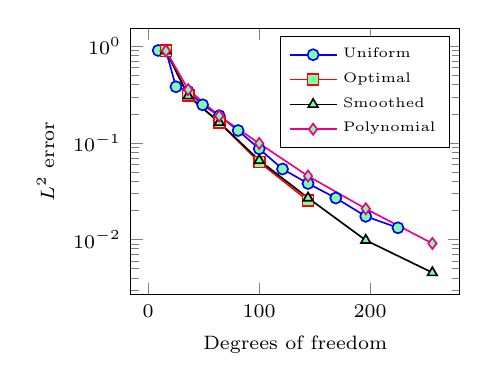
\begin{tikzpicture}
\begin{semilogyaxis}[
    legend cell align=left,
    legend style={legend pos=north east, font=\tiny},
    width=.475\textwidth,
    xlabel={Degrees of freedom},
    ylabel={$L^2$ error}, 
    grid style=dashed,
] 
\addplot[color=blue,mark=*,semithick, mark options={fill=markercolor}]
coordinates{(9,0.906971)(16,0.901137)(25,0.381376)(36,0.341234)(49,0.248105)(64,0.191363)(81,0.134334)(100,0.0867865)(121,0.0536073)(144,0.0379541)(169,0.0268356)(196,0.017334)(225,0.0131923)};

\addplot[color=red,mark=square*,semithick, mark options={fill=markercolor}]
coordinates{(16,0.899144)(36,0.311068)(64,0.16248)(100,0.063352)(144,0.0251876)};

\addplot[color=black,mark=triangle*,semithick, mark options={fill=markercolor}]
coordinates{(16,0.899144)(36,0.306762)(64,0.163124)(100,0.0659579)(144,0.0268692)(196,0.00979722)(256,0.00452463)};

\addplot[color=magenta,mark=diamond*,semithick, mark options={fill=markercolor}]
coordinates{(16,0.899144)(36,0.356753)(64,0.189946)(100,0.0987331)(144,0.0453151)(196,0.020774)(256,0.00908005)};

\legend{Uniform, Optimal, Smoothed, Polynomial}
\end{semilogyaxis}
\end{tikzpicture}
}
\caption{$L^2$ errors for $\cos\LRp{\frac{3\pi x}{2}}\cos\LRp{\frac{3\pi y}{2}}$ under degree refinement $N = 2,\ldots, 8$, using spline spaces with $K = N$ elements. }
}
\end{overlayarea}
\end{figure}
}

\frame{
\frametitle{Application to IGA and time-domain wave propagation}
\setcounter{subfigure}{0}

\begin{itemize}
\item Bound $\rho(\bm{A}_h)$ using generalized Rayleigh quotients (Bendixon-Hirsch): depends on $h$ and \textbf{constants} $C_T, C_I$.
\vspace{.5em}
\item CFL: $O(h/ N^2)$ for polynomials, $\textcolor{red}{O(h/ N)}$ for splines if $h \geq O(1/N)$.  
\end{itemize}
\vspace{-.5em}
\begin{figure}
\centering
\subfloat[Inverse inequality, $K = 2N$]{
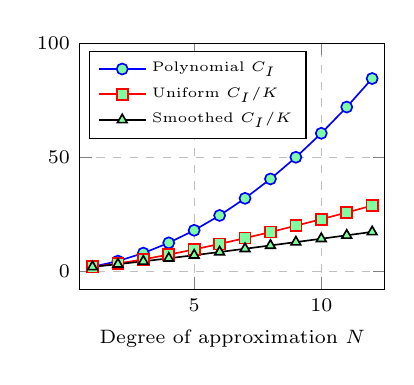
\begin{tikzpicture}
\begin{axis}[
width=.45\textwidth,
    xlabel={Degree of approximation $N$},   
    xmin=.5, xmax=12.5,
    ymax=0,ymax=100,    
    legend pos=north west, legend cell align=left, legend style={font=\tiny},	
    xmajorgrids=true,  ymajorgrids=true, grid style=dashed,
] 

\addplot[color=blue,mark=*,semithick, mark options={fill=markercolor}]
coordinates{(1,2)(2,4.5)(3,8)(4,12.5)(5,18)(6,24.5)(7,32)(8,40.5)(9,50)(10,60.5)(11,72)(12,84.5)};
\addplot[color=red,mark=square*,semithick, mark options={fill=markercolor}]
coordinates{(1,2)(2,3.42857)(3,5.27022)(4,7.3491)(5,9.61122)(6,12.0258)(7,14.5716)(8,17.233)(9,19.9977)(10,22.8559)(11,25.7995)(12,28.8217)};
\addplot[color=black,mark=triangle*,semithick, mark options={fill=markercolor}]
coordinates{(1,2)(2,3.15356)(3,4.41024)(4,5.72791)(5,7.09105)(6,8.48919)(7,9.91299)(8,11.3583)(9,12.8221)(10,14.3019)(11,15.796)(12,17.3028)};

\legend{Polynomial $C_I$, Uniform $C_I/K$, Smoothed $C_I/K$ }
\end{axis}
\end{tikzpicture}
}
\hspace{1em}
\subfloat[Trace inequality, $K = 2N$]{
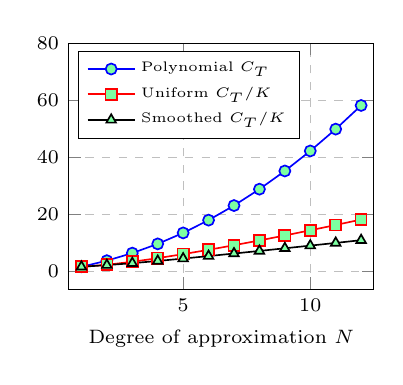
\begin{tikzpicture}
\begin{axis}[
width=.45\textwidth,
    xlabel={Degree of approximation $N$},   
    xmin=.5, xmax=12.5,
    ymax=0,ymax=80,    
    legend pos=north west, legend cell align=left, legend style={font=\tiny},	
    xmajorgrids=true,  ymajorgrids=true, grid style=dashed,
] 

\addplot[color=blue,mark=*,semithick, mark options={fill=markercolor}]
coordinates{(1,1.73205)(2,3.87298)(3,6.5216)(4,9.74981)(5,13.5914)(6,18.0596)(7,23.1598)(8,28.894)(9,35.2634)(10,42.2685)(11,49.9096)(12,58.187)};
\addplot[color=red,mark=square*,semithick, mark options={fill=markercolor}]
coordinates{(1,1.73205)(2,2.43668)(3,3.48657)(4,4.75661)(5,6.16327)(6,7.6751)(7,9.27477)(8,10.9506)(9,12.694)(10,14.4983)(11,16.3578)(12,18.2682)};
\addplot[color=black,mark=triangle*,semithick, mark options={fill=markercolor}]
coordinates{(1,1.73205)(2,2.32019)(3,2.9916)(4,3.77273)(5,4.61001)(6,5.4806)(7,6.37331)(8,7.28317)(9,8.20701)(10,9.14265)(11,10.0885)(12,11.0432)};

\legend{Polynomial $C_T$, Uniform $C_T / K $, Smoothed $C_T/K$ }
\end{axis}
\end{tikzpicture}
}
%\caption{Constants in spline inverse and trace inequalities for $K = 2N$.}
\end{figure}
}


\subsection{Elastic wave propagation}

\begin{frame}[noframenumbering]
    \frametitle{Outline}
    \tableofcontents[currentsection,currentsubsection]
\end{frame}


\frame{
\frametitle{Matrix-valued weights and elastic wave propagation}
\begin{itemize}
\item Symmetric velocity-stress form of linear elasticity ($\bm{A}_i$ constant)
\begin{align*}
\rho\pd{\bm{v}}{t}{} = \sum_{i=1}^d \bm{A}_i^T \pd{\bm{\sigma}}{\bm{x}_i}{}, \qquad \bm{C}^{-1}\pd{\bm{\sigma}}{t}{} = \sum_{i=1}^d \bm{A}_i \pd{\bm{v}}{\bm{x}_i}{}.
\end{align*}
\item DG formulation based on penalty fluxes, matrix-weighted mass matrix
\[
\LRp{\bm{M}_{\bm{C}^{-1}}}^{-1} = \LRp{\begin{array}{ccc}
\bm{M}_{C^{-1}_{11}} & \ldots & \bm{M}_{C^{-1}_{1d}}\\
\vdots & \ddots & \vdots\\
\bm{M}_{C^{-1}_{d1}} & \ldots & \bm{M}_{C^{-1}_{dd}}\\
\end{array}}
\]
%\begin{align*}
%\LRp{\rho\pd{\bm{v}}{t}{},\bm{w}} &= \LRp{\sum_{i=1}^d \bm{A}_i^T \pd{\bm{\sigma}}{\bm{x}_i}{},\bm{w} }+ \frac{1}{2}\LRa{\LRp{\bm{A}_n^T\jump{\bm{\sigma}} + \tau_v\bm{A}_n^T\bm{A}_n\jump{\bm{v}}},\bm{w}} \\
%\LRp{\bm{C}^{-1}\pd{\bm{\sigma}}{t}{}, \bm{q}}&= \LRp{\sum_{i=1}^d \bm{A}_i \pd{\bm{v}}{\bm{x}_i}{},\bm{q}} + \frac{1}{2}\LRa{\LRp{\bm{A}_n\jump{\bm{v}} + \tau_\sigma\bm{A}_n\bm{A}_n^T\jump{\bm{\sigma}}},\bm{q}} \\.
%\end{align*}
\item Weight-adjusted approximation for $\bm{C}^{-1}$ decouples into components 
\[
\bm{M}_{\bm{C}^{-1}}^{-1} \approx \LRp{\bm{I}\otimes \bm{M}^{-1}} \bm{M}_{\bm{C}} \LRp{\bm{I} \otimes\bm{M}^{-1}}.
\]
%\item Reduces to Kronecker product $\bm{M}_{\bm{C}^{-1}}^{-1} = \bm{C}^{-1}\otimes \bm{M}^{-1}$ for constant $\bm{C}^{-1}$.
\end{itemize}

\let\thefootnote\relax\footnotetext{\tiny Hughes and Marsden 1978. Classical elastodynamics as a linear symmetric hyperbolic system.}
}

\frame{
\frametitle{Elastic wave propagation: convergence}
\setcounter{subfigure}{0}
\begin{itemize}
\item Convergence for harmonic oscillation, Rayleigh, Lamb, and Stoneley waves: between $O(h^{N+1})$ and $O(h^{N+1/2})$.  
\vspace{1em}
\item $\bm{\sigma}$ error grows as $\nor{\bm{C}^{-1}}\rightarrow \infty$ (e.g.\ incompressible limit $\lambda/\mu \rightarrow \infty$).  
\end{itemize}
\vspace{-1em}
\begin{figure}
\centering
\subfloat[Stoneley wave]{
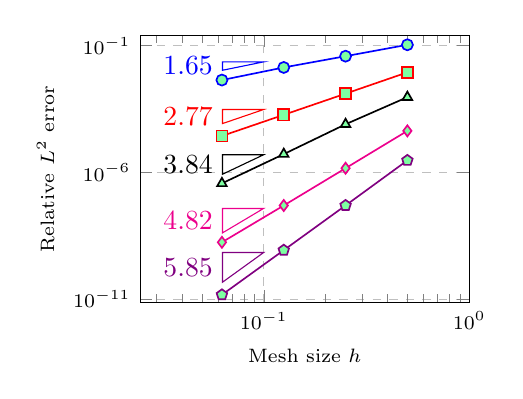
\begin{tikzpicture}
\begin{loglogaxis}[
    legend cell align=left,
    legend style={legend pos=south east, font=\tiny},
    width=.475\textwidth,
    xlabel={Mesh size $h$},
    ylabel={Relative $L^2$ error}, 
    xmin=.025, xmax=1,
    ymin=.75e-11, ymax=.25,
    xmajorgrids=true,
    ymajorgrids=true,
    grid style=dashed,
] 

\addplot[color=blue,mark=*,semithick, mark options={fill=markercolor}]
coordinates{(0.5,0.108456)(0.25,0.0385149)(0.125,0.0138288)(0.0625,0.0043988)};    
\logLogSlopeTriangleFlip{0.375}{0.125}{0.87}{1.65}{blue}

\addplot[color=red,mark=square*,semithick, mark options={fill=markercolor}]
coordinates{(0.5,0.00887301)(0.25,0.00128102)(0.125,0.000186756)(0.0625,2.73376e-05)};    
\logLogSlopeTriangleFlip{0.375}{0.125}{0.67}{2.77}{red}

\addplot[color=black,mark=triangle*,semithick, mark options={fill=markercolor}]
coordinates{(0.5,0.000930299)(0.25,7.92165e-05)(0.125,5.2534e-06)(0.0625,3.67676e-07)};    
\logLogSlopeTriangleFlip{0.375}{0.125}{0.48}{3.84}{black}

\addplot[color=magenta,mark=diamond*,semithick, mark options={fill=markercolor}]
coordinates{(0.5,4.34823e-05)(0.25,1.45784e-06)(0.125,4.92754e-08)(0.0625,1.74105e-09)};   
\logLogSlopeTriangleFlip{0.375}{0.125}{0.26}{4.82}{magenta}

\addplot[color=violet,mark=pentagon*,semithick, mark options={fill=markercolor}]
coordinates{(0.5,2.97005e-06)(0.25,4.94512e-08)(0.125,8.48451e-10)(0.0625,1.47109e-11)};  
\logLogSlopeTriangleFlip{0.375}{0.125}{0.075}{ 5.85}{violet}

%\node at (axis cs:.03,6.8e-10) {$u$ discontinuous};
%\legend{$N=1$,$N=2$,$N=3$,$N=4$,$N=5$}
\end{loglogaxis}
\end{tikzpicture}
}
\subfloat[$\nor{\bm{C^{-1}}}\rightarrow \infty$, $N=3, h = 1/8$.]{
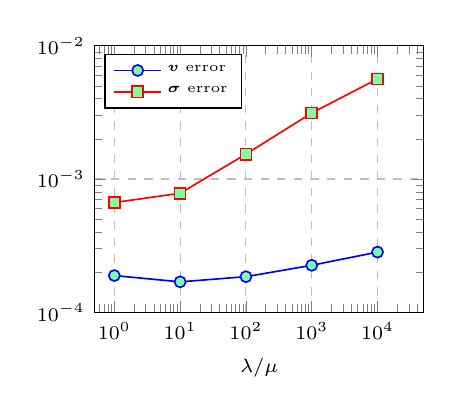
\begin{tikzpicture}
\begin{loglogaxis}[
    legend cell align=left,
    legend style={legend pos=north west, font=\tiny},
    width=.475\textwidth,
    xlabel={$\lambda / \mu$},
%    ylabel={Relative $L^2$ error}, 
    xmin=.5, xmax=5e4,
    ymin=1e-4, ymax=1e-2,
    xmajorgrids=true,
    ymajorgrids=true,
    grid style=dashed,
] 

\addplot[color=blue,mark=*,semithick, mark options={fill=markercolor}]
coordinates{(1,0.00018867)(10,0.00016925)(100,0.00018509)(1000,0.0002252)(10000,0.00028301)};

\addplot[color=red,mark=square*,semithick, mark options={fill=markercolor}]
coordinates{(1,0.00066596)(10,0.00078157)(100,0.0015353)(1000,0.0031239)(10000,0.0056341)};

\legend{$\bm{v}$ error, $\bm{\sigma}$ error }
\end{loglogaxis}
\end{tikzpicture}
}
\end{figure}
%\item Single precision energy stability 
}
%
%\frame{
%\frametitle{Elastic wave propagation: stiff inclusion}
%\begin{figure}
%\centering
%\includegraphics[width=.55\textwidth]{figs/inclusion_aligned.png}\\
%\includegraphics[width=.55\textwidth]{figs/inclusion_aligned_shear.png}
%\caption{Blah}
%\end{figure}
%}

\frame{
\frametitle{Elastic wave propagation: anisotropy}
\setcounter{subfigure}{0}
\vspace{.5em}
No change in implementation for anisotropy - fluxes independent of $\bm{C}$. 
\vspace{-.5em}
\begin{figure}
\centering
\subfloat[Vertical velocity, $t=30\mu s$]{\includegraphics[height=.525\textheight]{figs/aniso1.png}}
\subfloat[Vertical velocity, $t=60 \mu s$]{\includegraphics[height=.526\textheight]{figs/aniso2.png}}
\caption{Heterogeneous media: transverse isotropy ($x < 0$) and isotropy ($x > 0$).}
\end{figure}

\let\thefootnote\relax\footnotetext{\tiny Komatitsch, Barnes, Tromp 2000. Simulation of anisotropic wave propagation based upon a spectral element method.}
}

\frame{
\frametitle{Elastic wave propagation: acoustic-elastic coupling}
\setcounter{subfigure}{0}

\begin{itemize}
\item Interface jumps become residuals of continuity conditions:
\[
\bm{\sigma} \cdot \bm{n} = p\bm{n}, \qquad \bm{v}\cdot{\bm{n}} = \bm{u}\cdot\bm{n}.
\]
\item Energy stable for arbitrary heterogeneous media.  
\end{itemize}
\vspace{-.5em}
\begin{overlayarea}{\textwidth}{.65\textheight}
\begin{figure}
\centering
\only<1>{\subfloat[Low order $c^2(\bm{x}), \mu(\bm{x})$]{\includegraphics[width=.3825\textwidth]{figs/c2muP0.png}}
\hspace{1.5em}
\subfloat[${\rm tr}(\bm{\sigma})$]{\includegraphics[width=.4\textwidth]{figs/acousticElasticPulseP0.png}}
\caption{Acoustic-elastic waves from a Ricker pulse ($N=10$, $h = 1/16$).}
}

\only<2>{\subfloat[High order $c^2(\bm{x}), \mu(\bm{x})$]{\includegraphics[width=.3825\textwidth]{figs/c2mu.png}}
\hspace{1.5em}
\subfloat[${\rm tr}(\bm{\sigma})$]{\includegraphics[width=.4\textwidth]{figs/acousticElasticPulseP10.png}}
\caption{Acoustic-elastic waves from a Ricker pulse ($N=10$, $h = 1/16$).}
}

\end{figure}
\end{overlayarea}

\let\thefootnote\relax\footnotetext{\tiny Ye et al.\ 2016. A DG method with a modified penalty flux for the propagation and scattering of acousto-elastic waves.}
}

\frame{
\frametitle{Elastic wave propagation: 3D isotropic media}
\setcounter{subfigure}{0}
\begin{figure}
\begin{overlayarea}{\textwidth}{.75\textheight}
\centering
\only<1>{
\subfloat[Computational mesh]{\includegraphics[width=.475\textwidth]{figs/cubeSplitFine.png}}
\subfloat[Piecewise constant $\bm{C}(\bm{x})$]{\includegraphics[width=.475\textwidth]{figs/pplanec0.png}}
}
\only<2>{
\subfloat[High order $\bm{C}(\bm{x})$]{\includegraphics[width=.475\textwidth]{figs/pplanew0.png}}
\subfloat[Piecewise constant $\bm{C}(\bm{x})$]{\includegraphics[width=.475\textwidth]{figs/pplanec0.png}}
}
\end{overlayarea}
\caption{${\rm tr}(\bm{\sigma})$ with $\mu(\bm{x}) = 1+ H(y) + \frac{1}{2}\cos(3\pi x)\cos(3\pi y)\cos(3\pi z)$, $N=5$.}
\end{figure}
}

\frame{
\frametitle{Summary and acknowledgements}

\begin{itemize}
\item \textbf{Sparsity} of Bernstein-Bezier DG: efficiency at high orders on GPUs.
\vspace{1em}
\item Weight-adjusted DG (WADG): low-storage methods for heterogeneous media and curvilinear meshes.
\vspace{1em}
\item Future work: 
\vspace{.5em}
\begin{itemize}
\item Exploit structure of WADG under Bernstein-Bezier basis.  
\vspace{.5em}
\item WADG with singular weights.
\end{itemize}
\end{itemize}
\vspace{.5em}
\begin{center}
Thanks to TOTAL E\&P Research and Technology USA\\ for their support of this work.
\end{center}

\let\thefootnote\relax\footnotetext{\tiny Chan 2017.  Weight-adjusted DG methods: matrix-valued weights and elastic wave prop.\ in heterogeneous media (arXiv).}
\let\thefootnote\relax\footnotetext{\tiny Chan, et al.\ 2016.  {Weight-adjusted DG methods: wave propagation in heterogeneous media} (arXiv).}
\let\thefootnote\relax\footnotetext{\tiny Chan, et al.\ 2016.  {Weight-adjusted DG methods: curvilinear meshes} (arXiv).  }
\let\thefootnote\relax\footnotetext{\tiny Chan, Warburton 2015. {GPU-accelerated Bernstein-Bezier DG methods for wave problems} (SISC).}
}

%\frame{
%\begin{center}
%The authors thank TOTAL E\&P Research and Technology USA\\
%for their generous support of this work.
%\end{center}
%\let\thefootnote\relax\footnotetext{\tiny Chan, Warburton 2015. {GPU-accelerated Bernstein-Bezier DG methods for wave problems}.}
%\let\thefootnote\relax\footnotetext{\tiny Chan, Warburton 2015.  A short note on a Bernstein-Bezier basis for the pyramid.  (SISC, accepted)}
%\let\thefootnote\relax\footnotetext{\tiny Chan, et al.\ 2016.  {WADG methods I: wave propagation in heterogeneous media}.  In preparation.}
%\let\thefootnote\relax\footnotetext{\tiny Chan, et al.\ 2016.  {WADG methods II: curvilinear meshes}.  In preparation.}
%}
%% =================== extra slides =======================

\begin{frame}[noframenumbering]
\frametitle{Additional slides }
\end{frame}


\frame[noframenumbering]{
\frametitle{Roofline model: estimating computational efficiency} %peak performance ``ceilings''}
%\vspace{-.5em}
\begin{itemize}
%\item Why are nodal tetrahedra slower at high orders?
\item Arithmetic intensity: floating-point operations per byte of data.
%\only<2>{
%\item Additional ``ceilings'' from unrealized optimizations.
\item Computational efficiency: ratio of observed/achievable performance.
%}
\end{itemize}
\vspace{-1em}
\begin{figure}
\centering
%\only<1>{\includegraphics[width=.65\textwidth]{figs/rooflineGraph.pdf}}%
%\only<2>{\includegraphics[width=.65\textwidth]{figs/rooflineGraph1.pdf}}%
\only<1>{\includegraphics[width=.65\textwidth]{figs/roofline1.pdf}}%
\only<2>{\includegraphics[width=.65\textwidth]{figs/roofline2.pdf}}%
\only<3>{\includegraphics[width=.65\textwidth]{figs/roofline3.pdf}}%
%\only<1>{\includegraphics[width=.65\textwidth]{figs/rooflineGraph.pdf}}%
%\only<2>{\includegraphics[width=.65\textwidth]{figs/rooflineGraph1.pdf}}%
%\only<3>{\includegraphics[width=.65\textwidth]{figs/rooflineGraph2.pdf}}%
\end{figure}
\vspace{-1em}
\let\thefootnote\relax\footnotetext{\tiny Williams, Waterman, Patterson 2009. Roofline: an insightful visual performance model for multicore architectures.}
}

\frame[noframenumbering]{
\frametitle{Performance comparisons of Bernstein-Bezier DG}
%\begin{itemize}
%\item 
\vspace{.25em}
Bernstein-Bezier DG: standard implementation, sparse matrices.  
\[
\underbrace{\td{\bm{u}}{t}}_{\text{Update kernel}} = \underbrace{\mathbf{D}_x \mathbf{u}}_{\text{Volume kernel}} + \underbrace{\sum_{\text{ faces}}\mathbf{L}_f \LRp{\rm flux}}_{\text{Surface kernel}}, \quad \mathbf{L}_f = \mathbf{{M}}^{-1}\mathbf{{M}}_f.
\]
%\item We compare Bernstein-Bezier DG with standard and optimized block-partitioned implementations of nodal DG.  
%\end{itemize}
\vspace{-1em}
\begin{figure}
\centering
\begin{overlayarea}{\textwidth}{.75\textheight}
\subfloat{
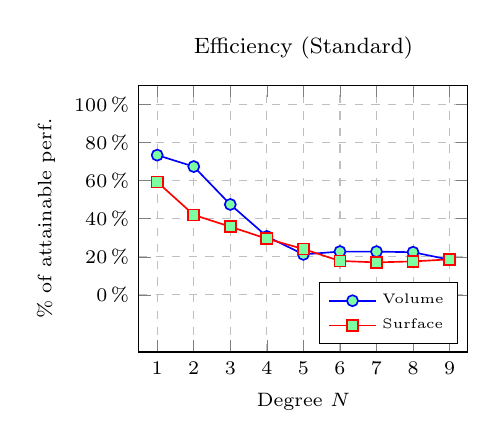
\begin{tikzpicture}
\begin{axis}[
 	legend cell align=left,
legend style={font=\tiny},		
	width=.475\textwidth,
%	title={Efficiency (Naive)},
	title={Efficiency (Standard)},
	xlabel={Degree $N$},
	ylabel={\% of attainable perf.},
	xmin=.5, xmax=9.5,
	ymin=-30, ymax=110,
	ytick = {0,20,40,60,80,100},
	xtick={1,2,3,4,5,6,7,8,9},	
	yticklabel=\pgfmathparse{\tick}\pgfmathprintnumber{\pgfmathresult}\,\%,
	legend pos=south east,
	xmajorgrids=true,
	ymajorgrids=true,
	grid style=dashed,
] 
%nodal efficiency
\addplot+[color=blue,mark=*,semithick,mark options={fill=markercolor}]
coordinates{(1,73.3937)(2,67.3929)(3,47.4955)(4,30.7009)(5,21.275)(6,22.7515)(7,22.7385)(8,22.4154)(9,18.4931)};
\addplot+[color=red,mark=square*,semithick,mark options={fill=markercolor}]
coordinates{(1,59.3125)(2,42.0089)(3,35.817)(4,29.4969)(5,24.096)(6,17.8277)(7,17.078)(8,17.5887)(9,18.6729)};
\legend{Volume, Surface}
\end{axis}
\end{tikzpicture}
}
\subfloat{
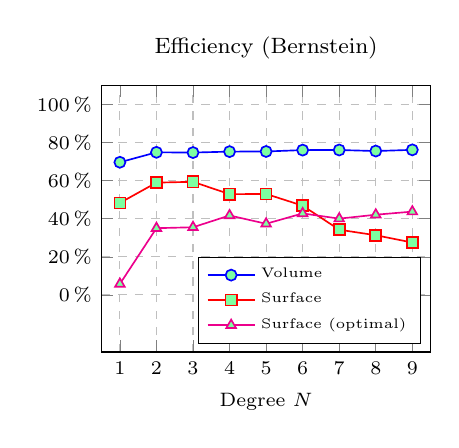
\begin{tikzpicture}
\begin{axis}[
	legend cell align=left,
legend style={font=\tiny},	
	width=.475\textwidth,
    title={Efficiency (Bernstein)},
    xlabel={Degree $N$},
    xmin=.5, xmax=9.5,
    ymin=-30, ymax=110,
    ytick = {0,20,40,60,80,100},
	xtick={1,2,3,4,5,6,7,8,9},    
    yticklabel=\pgfmathparse{\tick}\pgfmathprintnumber{\pgfmathresult}\,\%,
    legend pos=south east,
    xmajorgrids=true,   
    ymajorgrids=true,    
    grid style=dashed,
] 
%bern efficiency

\addplot+[color=blue,mark=*,semithick,mark options={fill=markercolor}]
coordinates{(1,69.6554)(2,74.8705)(3,74.7451)(4,75.2384)(5,75.3134)(6,76.0375)(7,76.0844)(8,75.5446)(9,76.1647)};

\addplot+[color=red,mark=square*,semithick,mark options={fill=markercolor}]
coordinates{(1,48.3089)(2,58.9629)(3,59.3893)(4,52.892)(5,53.0138)(6,46.8504)(7,34.2272)(8,31.3295)(9,27.5054)};

\addplot+[color=magenta,mark=triangle*,semithick,mark options={fill=markercolor}]
coordinates{(1,5.76161)(2,35.0402)(3,35.5219)(4,41.7219)(5,37.3567)(6,42.7942)(7,40.0491)(8,42.1121)(9,43.7357)};

\legend{Volume, Surface, Surface (optimal)}

\end{axis}
\end{tikzpicture}
}

\end{overlayarea}
\end{figure}
}


\frame[noframenumbering]{
\frametitle{Bernstein-Bezier compared to CUBLAS}
\vspace{-.5em}
\begin{center}
Bernstein-Bezier DG achieves $\approx 4\times$ speedup at low-moderate orders,\\ and $1.5-2\times$ speedup at high orders.
\end{center}
%\begin{center}
%Bernstein-Bezier DG achieves $\approx 2\times$ speedup at moderate orders,\\ and up to $4\times$ speedup at high orders.
%\end{center}
\vspace{-1em}
\begin{figure}
\centering
\only<1>{
\subfloat{
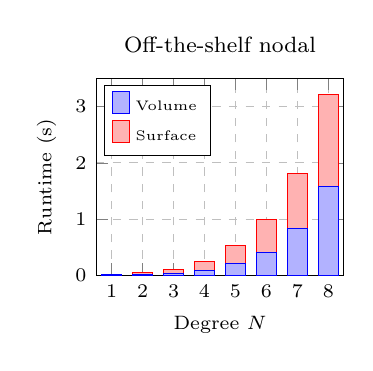
\begin{tikzpicture}
\begin{axis}[
	width=.39\textwidth,
	legend cell align=left,
	title={Off-the-shelf nodal},
	xlabel={Degree $N$},
	ylabel={Runtime (s)},
	xmin=.5, xmax=8.5,
	ymin=0,ymax=3.5,
	ybar stacked,
	    bar width=7pt,
	legend style={font=\tiny},	
	xtick={1,2,3,4,5,6,7,8},
	legend pos=north west,
	xmajorgrids=true,
	ymajorgrids=true,
	grid style=dashed,
] 
%nodal runtimes
\addplot coordinates{(1,0.00529)(2,0.0135)(3,0.0302)(4,0.0854)(5,0.206)(6,0.41)(7,0.829)(8,1.58)(9,3.39)};
\addplot coordinates{(1,0.0121)(2,0.0403)(3,0.0722)(4,0.158)(5,0.322)(6,0.587)(7,0.987)(8,1.64)(9,2.51)};
%\addplot coordinates{(1,0.009394)(2,0.025607)(3,0.046205)(4,0.080841)(5,0.142045)(6,0.19389)(7,0.27628)(8,0.381)(9,0.5088)};

\legend{Volume, Surface}%, Update}

\end{axis}
\end{tikzpicture}
}
\subfloat{
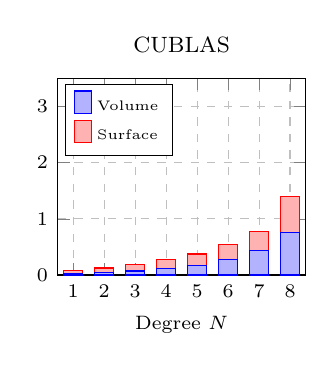
\begin{tikzpicture}
\begin{axis}[
	width=.39\textwidth,
	legend cell align=left,
	%title={Node-per-thread (NPT) nodal},
	%title={Naive nodal},
	title={CUBLAS},
	xlabel={Degree $N$},
%	ylabel={Runtime (s)},
	xmin=.5, xmax=8.5,
	ymin=0,ymax=3.5,
	ybar stacked,
        bar width=7pt,
	legend style={font=\tiny},	
%	nodes near coords,
	%xmin=.5, xmax=9.5,
	xtick={1,2,3,4,5,6,7,8},
	legend pos=north west,
	xmajorgrids=true,
	ymajorgrids=true,
	grid style=dashed,
] 
%nodal runtimes

\addplot coordinates{(1,0.0215)(2,0.0395)(3,0.072)(4,0.109)(5,0.171)(6,0.271)(7,0.441)(8,0.7505)};
\addplot coordinates{(1,0.052)(2,0.0855)(3,0.123)(4,0.172)(5,0.2025)(6,0.278)(7,0.335)(8,0.646)};
%\addplot coordinates{(1,0.009394)(2,0.025607)(3,0.046205)(4,0.080841)(5,0.142045)(6,0.19389)(7,0.27628)(8,0.381)(9,0.5088)};

\legend{Volume, Surface}%, Update}

\end{axis}
\end{tikzpicture}
}
\subfloat{
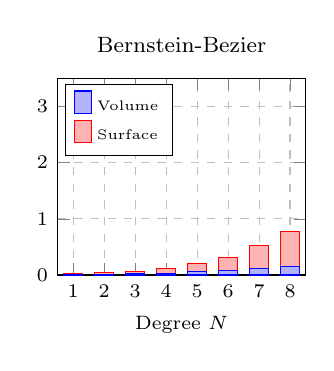
\begin{tikzpicture}
\begin{axis}[
	width=.39\textwidth,
	legend cell align=left,
	title={Bernstein-Bezier},
	xlabel={Degree $N$},
	legend style={font=\tiny},	
%	ylabel={Runtime (s)},
	xmin=.5, xmax=8.5,
	ymin=0,ymax=3.5,
	ybar stacked,
	    bar width=7pt,
	xtick={1,2,3,4,5,6,7,8},
	legend pos=north west,
	xmajorgrids=true,
	ymajorgrids=true,
	grid style=dashed,
] 
%bern runtimes
\addplot 
coordinates{(1,0.00564)(2,0.0119)(3,0.0203)(4,0.034)(5,0.0593)(6,0.0791)(7,0.112)(8,0.155)(9,0.204)};
\addplot 
coordinates{(1,0.0148)(2,0.0276)(3,0.0459)(4,0.0842)(5,0.149)(6,0.227)(7,0.42)(8,0.614)(9,0.912)};
%\addplot 
%coordinates{(1,0.0093767)(2,0.0255921)(3,0.04623)(4,0.081)(5,0.14229)(6,0.194133)(7,0.277041)(8,0.38163)(9,0.50694)};

\legend{Volume, Surface}%, Update}

\end{axis}
\end{tikzpicture}
}
%\caption*{Per-kernel runtimes for nodal and Bernstein-Bezier bases.  Runtimes are recorded for ten RK4 timesteps on a mesh of 98304 elements.}
%\caption*{Kernel runtimes for Naive nodal, Blocked nodal, and Bernstein-Bezier DG implementations (50 RHS evaluations, 98304 elements).}
%\caption*{Kernel runtimes for Standard nodal, Blocked nodal, and Bernstein-Bezier DG implementations (50 RHS evaluations, 98304 elements).}
%\caption*{DG runtimes for 50 timesteps, 98304 elements.}
}

% maybe comment out? speedup
\only<2>{
\subfloat{
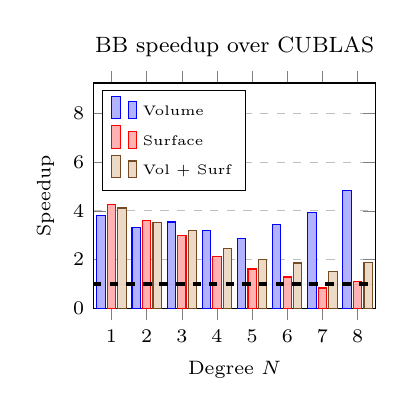
\begin{tikzpicture}
\begin{axis}[
	width=.425\textwidth,
	legend cell align=left,
	%title={BB speedup over Naive nodal},
	title={BB speedup over CUBLAS},
	xlabel={Degree $N$},
	ylabel={Speedup},
	xmin=.5, xmax=8.5,
	ymin=0,ymax=9.25,%17.5,	
        ybar=2*\pgflinewidth,
        bar width=3pt,
	xtick={1,2,3,4,5,6,7,8},
	ymin=0,
	legend pos=north west,
	legend style={font=\tiny},
	ymajorgrids=true,
	grid style=dashed,
] 
%speedup V/S
\addplot coordinates{(1,3.81206)(2,3.31933)(3,3.5468)(4,3.20588)(5,2.88364)(6,3.42604)(7,3.9375)(8,4.84194)};
\addplot coordinates{(1,4.2623)(2,3.62288)(3,3)(4,2.14732)(5,1.61741)(6,1.28823)(7,0.837709)(8,1.10465)};
\addplot coordinates{(1,4.11996)(2,3.52113)(3,3.18108)(4,2.46275)(5,2.02439)(6,1.86165)(7,1.51592)(8,1.88767)};
\addplot+[draw=black,line legend, very thick,smooth,dashed] coordinates{(0,1)(10,1)};
%\legend{Volume, Surface, Total, Reference (no speedup)}
\legend{Volume, Surface, Vol + Surf}%, No speedup}
\end{axis}
\end{tikzpicture}
}

%\caption*{Ratio of runtimes of volume/surface kernels and total RHS evaluation using a Bernstein-Bezier basis instead of nodal polynomials.}
%\caption*{Speedups achieved over nodal DG by using a Bernstein-Bezier basis.}
}
%\caption*{Bernstein-Bezier DG achieves $\approx 2\times$ speedup at moderate orders,\\ and up to $4\times$ speedup at high orders.}
\end{figure}
\only<1>{\vspace{-.25em}}
\only<2>{\vspace{-.5em}}
\[
\underbrace{\td{\mathbf{u}}{t}}_{\text{Update kernel}} = \underbrace{\mathbf{D}_x \mathbf{u}}_{\text{Volume kernel}} + \underbrace{\sum_{\text{ faces}}\mathbf{L}_f \LRp{\rm flux}}_{\text{Surface kernel}}, \quad \mathbf{L}_f = \mathbf{{M}}^{-1}\mathbf{{M}}_f.
\]


}

\frame[noframenumbering]{
\frametitle{Performance comparisons of Bernstein-Bezier DG}
\begin{figure}
\centering
\only<1>{
\subfloat{
\begin{tikzpicture}
\begin{axis}[
	width=.5\textwidth,
	legend cell align=left,
	legend style={font=\tiny},
	legend image post style={scale=0.5},
	title={Performance (Nodal)},
	xlabel={Degree $N$},
	ylabel={TFLOPS/s},
	xmin=.5, xmax=9.5,
	ymin=0,ymax=1.200,
        ybar=2*\pgflinewidth,
    bar width=3pt,
	%xmin=.5, xmax=9.5,
	xtick={1,2,3,4,5,6,7,8,9},
	ytick={0,.5,1,1.5,2},
	legend pos=north west,
%	xmajorgrids=true,
	ymajorgrids=true,
	grid style=dashed,
] 
\addplot table[x=N, y=V] from \GFLOPSNodal;
\addplot table[x=N, y=S] from \GFLOPSNodal;
\legend{Volume, Surface}
\end{axis}
\end{tikzpicture}
}
%\subfloat{
%\begin{tikzpicture}
%\begin{axis}[
%	width=.36\textwidth,
%	legend cell align=left,
%	legend style={font=\tiny},
%	legend image post style={scale=0.5},
%	title={Performance (EPT nodal)},
%	xlabel={Degree $N$},
%%	ylabel={GFLOPS/s},
%	xmin=.5, xmax=9.5,
%	ymin=0,ymax=2.500,
%        ybar=2*\pgflinewidth,
%    bar width=2pt,
%	%xmin=.5, xmax=9.5,
%	xtick={1,2,3,4,5,6,7,8,9},
%	ytick={0,.5,1,1.5,2},	
%	legend pos=north west,
%%	xmajorgrids=true,
%	ymajorgrids=true,
%	grid style=dashed,
%] 
%\addplot table[x=N, y=V] from \GFLOPSBlockNodal;
%\addplot table[x=N, y=S] from \GFLOPSBlockNodal;
%\addplot table[x=N, y=F] from \GFLOPSBlockNodal;
%\legend{Volume, Lift, Flux}
%
%\end{axis}
%\end{tikzpicture}
%}
\subfloat{
\begin{tikzpicture}
\begin{axis}[
	width=.5\textwidth,
	legend cell align=left,
	legend style={font=\tiny},
	legend image post style={scale=0.5},
	title={Performance (Bernstein)},
	xlabel={Degree $N$},
%	ylabel={GFLOPS/s},
	xmin=.5, xmax=9.5,
	ymin=0,ymax=1.2,
        ybar=2*\pgflinewidth,
    bar width=3pt,
	xtick={1,2,3,4,5,6,7,8,9},
	ytick={0,.5,1,1.5,2},	
	legend pos=north west,
%	xmajorgrids=true,
	ymajorgrids=true,
	grid style=dashed,
] 
\addplot table[x=N, y=V] from \GFLOPSBern;
\addplot table[x=N, y=S] from \GFLOPSBern;
\addplot table[x=N, y=L] from \GFLOPSBern;
\legend{Volume, Surface, Surface (optimal)}
\end{axis}
\end{tikzpicture}
}
}
\only<2>{
\subfloat{
\begin{tikzpicture}
\begin{axis}[
	width=.5\textwidth,
	legend cell align=left,
	legend style={font=\tiny},
	legend image post style={scale=0.5},	
	title={Bandwidth (Nodal)},
	xlabel={Degree $N$},
	ylabel={GB/s},
	xmin=.5, xmax=9.5,
	ymin=0,ymax=270,
        ybar=2*\pgflinewidth,
    bar width=3pt,
	%xmin=.5, xmax=9.5,
	xtick={1,2,3,4,5,6,7,8,9},
	legend pos=north east,
%	xmajorgrids=true,
	ymajorgrids=true,
	grid style=dashed,
] 
%nodal BW
\addplot table[x=N, y=V] from \BWNodal;
\addplot table[x=N, y=S] from \BWNodal;
\legend{Volume, Surface}

\end{axis}
\end{tikzpicture}
}
%\subfloat{
%\begin{tikzpicture}
%\begin{axis}[
%	width=.355\textwidth,
%	legend cell align=left,
%	legend style={font=\tiny},
%	legend image post style={scale=0.5},
%	title={Bandwidth (EPT nodal)},
%	xlabel={Degree $N$},
%	xmin=.5, xmax=9.5,
%	ymin=0,ymax=260,
%        ybar=2*\pgflinewidth,
%    bar width=1.75pt,
%	xtick={1,2,3,4,5,6,7,8,9},
%	legend pos=north east,
%	ymajorgrids=true,
%	grid style=dashed,
%] 
%%nodal BW
%\addplot table[x=N, y=V] from \BWBlockNodal;
%\addplot table[x=N, y=S] from \BWBlockNodal;
%\addplot table[x=N, y=F] from \BWBlockNodal;
%\legend{Volume, Lift, Flux}
%
%\end{axis}
%\end{tikzpicture}
%}
\subfloat{
\begin{tikzpicture}
\begin{axis}[
	width=.5\textwidth,
	legend cell align=left,
	legend style={font=\tiny},
	legend image post style={scale=0.5},	
	title={Bandwidth (Bernstein)},
	xlabel={Degree $N$},
	xmin=.5, xmax=9.5,
	ymin=0,ymax=270,
        ybar=2*\pgflinewidth,
    bar width=3pt,
	xtick={1,2,3,4,5,6,7,8,9},
	legend pos=north east,
	ymajorgrids=true,
	grid style=dashed,
] 

%bern BW
\addplot table[x=N, y=V] from \BWBern;
\addplot table[x=N, y=S] from \BWBern;
\addplot table[x=N, y=L] from \BWBern;
\legend{Volume, Surface, Surface (optimal)}
\end{axis}
\end{tikzpicture}
}
}
\end{figure}
}



\frame{
\frametitle[noframenumbering]{Preliminary comparisons: BBDG, SEM-DG on GPUs}
\vspace{-1.5em}
\begin{figure}
\begin{overlayarea}{\textwidth}{.6\textheight}
\centering
\only<1>{
\subfloat{
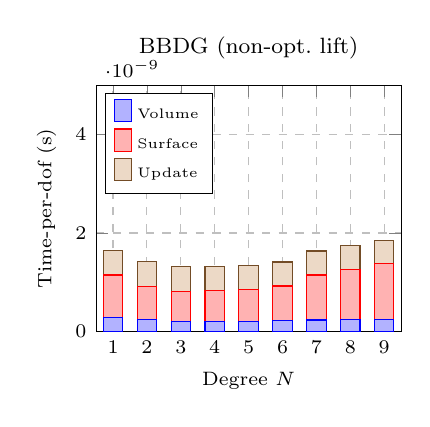
\begin{tikzpicture}
\begin{axis}[
	width=.45\textwidth,
	legend cell align=left,
	title={BBDG (non-opt.\ lift)},
	xlabel={Degree $N$},
	legend style={font=\tiny},	
	ylabel={Time-per-dof (s)},
	xmin=.5, xmax=9.5,
	ymin=0,ymax=5e-9,
	ybar stacked,
	bar width=7pt,
	xtick={1,2,3,4,5,6,7,8,9},
	legend pos=north west,
	xmajorgrids=true,
	ymajorgrids=true,
	grid style=dashed,
] 
%bern runtimes
\addplot 
coordinates{(1,2.83e-10)(2,2.37e-10)(3,2.09e-10)(4,2.07e-10)(5,1.96e-10)(6,2.22e-10)(7,2.33e-10)(8,2.47e-10)(9,2.43e-10)(10,2.64e-10)};
\addplot 
coordinates{(1,8.65e-10)(2,6.81e-10)(3,6.11e-10)(4,6.32e-10)(5,6.56e-10)(6,7.01e-10)(7,9.14e-10)(8,1.02e-09)(9,1.13e-09)(10,1.42e-09)};
\addplot 
coordinates{(1,4.97e-10)(2,5.09e-10)(3,4.99e-10)(4,4.83e-10)(5,4.89e-10)(6,4.88e-10)(7,4.87e-10)(8,4.81e-10)(9,4.8e-10)(10,4.78e-10)};
\legend{Volume, Surface, Update}

\end{axis}
\end{tikzpicture}
}
\hspace{1em}
\subfloat{
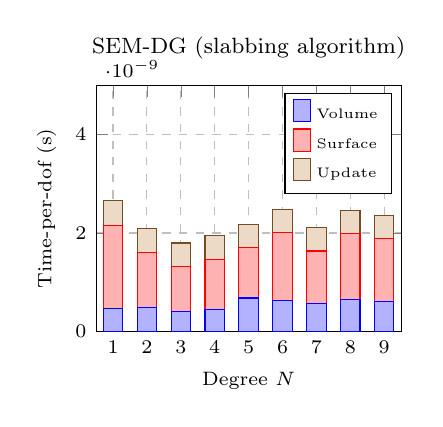
\begin{tikzpicture}
\begin{axis}[
	width=.45\textwidth,
	legend cell align=left,
	title={SEM-DG (slabbing algorithm)},
	xlabel={Degree $N$},
	legend style={font=\tiny},	
	ylabel={Time-per-dof (s)},
	xmin=.5, xmax=9.5,
	ymin=0,ymax=5e-9,
	ybar stacked,
	bar width=7pt,
	xtick={1,2,3,4,5,6,7,8,9},
	legend pos=north east,
	xmajorgrids=true,
	ymajorgrids=true,
	grid style=dashed,
] 
%bern runtimes
\addplot 
coordinates{(1,4.6e-10)(2,4.92e-10)(3,4.14e-10)(4,4.45e-10)(5,6.8e-10)(6,6.32e-10)(7,5.74e-10)(8,6.43e-10)(9,6.1e-10)(10,6.19e-10)};
\addplot 
coordinates{(1,1.69e-09)(2,1.12e-09)(3,9.06e-10)(4,1.02e-09)(5,1.02e-09)(6,1.37e-09)(7,1.06e-09)(8,1.35e-09)(9,1.27e-09)(10,1.22e-09)};
\addplot 
coordinates{(1,5.13e-10)(2,4.87e-10)(3,4.77e-10)(4,4.82e-10)(5,4.81e-10)(6,4.75e-10)(7,4.71e-10)(8,4.73e-10)(9,4.81e-10)(10,4.81e-10)};
\legend{Volume, Surface, Update}

\end{axis}
\end{tikzpicture}
}
}
\only<2>{
\subfloat{\includegraphics[width=.6\textwidth]{figs/hex_nodes.eps}}
}
\end{overlayarea}

\end{figure}
\vspace{-1em}
\begin{itemize}
%\item SEM-DG asymptotic complexity $O(N^4)$ (negligible for $N = O(10)$).
\item BBDG 1-1.75$\times$ faster per dof than SEM-DG for $N \leq 10$.
\item Unstructured hex meshes: \only<1>{$9(N+1)^3$}\only<2>{\textcolor{red}{$9(N+1)^3$}} geometric factors per element.
\item Disclaimer: hexes are more accurate, need time-to-error studies!  
\end{itemize}
\let\thefootnote\relax\footnotetext{\tiny Abdi, Wilcox, Warburton, Giraldo 2016.  A GPU Accel.\ Cont.\ and Disc.\ Galerkin Non-hydrostatic Atmospheric Model}
}

\frame[noframenumbering]{
\frametitle{Effect of conservation on shock speeds}

\begin{itemize}
\item Weighted Burgers' equation, $w(x)$ curves characteristic lines.
\[
w(x)\pd{u}{t}{} + \frac{1}{2}\pd{u^2}{x}{} = 0.
\]
\item WADG yields high order convergence, correct shock speed for both $w(x)$ smooth, discontinuous (within an element).
\end{itemize}
%\vspace{-1em}
\begin{overlayarea}{\textwidth}{.55\textheight}
\only<1>{
\begin{figure}
\centering
\subfloat[Smooth solution]{\includegraphics[width=.4\textwidth]{figs/burgersSmooth2.png}}
\hspace{1em}
\subfloat[Shock solution]{\includegraphics[width=.39\textwidth]{figs/burgersShock2.png}}
\end{figure}
}
\only<2>{
\vspace{2em}
\begin{center}
Best guess: {where} and {what} is locally conserved matters;\\ non-conservation of \textit{nonlinear flux} results in incorrect shock speeds.  
\end{center}
}
\end{overlayarea}
}


\bibliographystyle{plain}
{\scriptsize
\bibliography{pyramids}
}

\end{document}
